\documentclass[11pt,a4paper,]{article}
\usepackage{lmodern}

\usepackage{amssymb,amsmath}
\usepackage{ifxetex,ifluatex}
\usepackage{fixltx2e} % provides \textsubscript
\ifnum 0\ifxetex 1\fi\ifluatex 1\fi=0 % if pdftex
  \usepackage[T1]{fontenc}
  \usepackage[utf8]{inputenc}
\else % if luatex or xelatex
  \usepackage{unicode-math}
  \defaultfontfeatures{Ligatures=TeX,Scale=MatchLowercase}
\fi
% use upquote if available, for straight quotes in verbatim environments
\IfFileExists{upquote.sty}{\usepackage{upquote}}{}
% use microtype if available
\IfFileExists{microtype.sty}{%
\usepackage[]{microtype}
\UseMicrotypeSet[protrusion]{basicmath} % disable protrusion for tt fonts
}{}
\PassOptionsToPackage{hyphens}{url} % url is loaded by hyperref
\usepackage[unicode=true]{hyperref}
\hypersetup{
            pdftitle={Peeking inside FFORMS: Feature-based FORecast Model Selection},
            pdfkeywords={forecasting, time series, machine learning interpretability, black-box models, LIME},
            pdfborder={0 0 0},
            breaklinks=true}
\urlstyle{same}  % don't use monospace font for urls
\usepackage{geometry}
\geometry{left=2.5cm,right=2.5cm,top=2.5cm,bottom=2.5cm}
\usepackage[style=authoryear-comp,]{biblatex}
\addbibresource{references.bib}
\usepackage{longtable,booktabs}
% Fix footnotes in tables (requires footnote package)
\IfFileExists{footnote.sty}{\usepackage{footnote}\makesavenoteenv{long table}}{}
\usepackage{graphicx,grffile}
\makeatletter
\def\maxwidth{\ifdim\Gin@nat@width>\linewidth\linewidth\else\Gin@nat@width\fi}
\def\maxheight{\ifdim\Gin@nat@height>\textheight\textheight\else\Gin@nat@height\fi}
\makeatother
% Scale images if necessary, so that they will not overflow the page
% margins by default, and it is still possible to overwrite the defaults
% using explicit options in \includegraphics[width, height, ...]{}
\setkeys{Gin}{width=\maxwidth,height=\maxheight,keepaspectratio}
\IfFileExists{parskip.sty}{%
\usepackage{parskip}
}{% else
\setlength{\parindent}{0pt}
\setlength{\parskip}{6pt plus 2pt minus 1pt}
}
\setlength{\emergencystretch}{3em}  % prevent overfull lines
\providecommand{\tightlist}{%
  \setlength{\itemsep}{0pt}\setlength{\parskip}{0pt}}
\setcounter{secnumdepth}{5}

% set default figure placement to htbp
\makeatletter
\def\fps@figure{htbp}
\makeatother


\title{Peeking inside FFORMS: Feature-based FORecast Model Selection}

%% MONASH STUFF

%% CAPTIONS
\RequirePackage{caption}
\DeclareCaptionStyle{italic}[justification=centering]
 {labelfont={bf},textfont={it},labelsep=colon}
\captionsetup[figure]{style=italic,format=hang,singlelinecheck=true}
\captionsetup[table]{style=italic,format=hang,singlelinecheck=true}

%% FONT
\RequirePackage{bera}
\RequirePackage{mathpazo}

%% HEADERS AND FOOTERS
\RequirePackage{fancyhdr}
\pagestyle{fancy}
\rfoot{\Large\sffamily\raisebox{-0.1cm}{\textbf{\thepage}}}
\makeatletter
\lhead{\textsf{\expandafter{\@title}}}
\makeatother
\rhead{}
\cfoot{}
\setlength{\headheight}{15pt}
\renewcommand{\headrulewidth}{0.4pt}
\renewcommand{\footrulewidth}{0.4pt}
\fancypagestyle{plain}{%
\fancyhf{} % clear all header and footer fields
\fancyfoot[C]{\sffamily\thepage} % except the center
\renewcommand{\headrulewidth}{0pt}
\renewcommand{\footrulewidth}{0pt}}

%% MATHS
\RequirePackage{bm,amsmath}
\allowdisplaybreaks

%% GRAPHICS
\RequirePackage{graphicx}
\setcounter{topnumber}{2}
\setcounter{bottomnumber}{2}
\setcounter{totalnumber}{4}
\renewcommand{\topfraction}{0.85}
\renewcommand{\bottomfraction}{0.85}
\renewcommand{\textfraction}{0.15}
\renewcommand{\floatpagefraction}{0.8}

%\RequirePackage[section]{placeins}

%% SECTION TITLES
\RequirePackage[compact,sf,bf]{titlesec}
\titleformat{\section}[block]
  {\fontsize{15}{17}\bfseries\sffamily}
  {\thesection}
  {0.4em}{}
\titleformat{\subsection}[block]
  {\fontsize{12}{14}\bfseries\sffamily}
  {\thesubsection}
  {0.4em}{}
\titlespacing{\section}{0pt}{*5}{*1}
\titlespacing{\subsection}{0pt}{*2}{*0.2}


%% TITLE PAGE
\def\Date{\number\day}
\def\Month{\ifcase\month\or
 January\or February\or March\or April\or May\or June\or
 July\or August\or September\or October\or November\or December\fi}
\def\Year{\number\year}

\makeatletter
\def\wp#1{\gdef\@wp{#1}}\def\@wp{??/??}
\def\jel#1{\gdef\@jel{#1}}\def\@jel{??}
\def\showjel{{\large\textsf{\textbf{JEL classification:}}~\@jel}}
\def\nojel{\def\showjel{}}
\def\addresses#1{\gdef\@addresses{#1}}\def\@addresses{??}
\def\cover{{\sffamily\setcounter{page}{0}
        \thispagestyle{empty}
        \placefig{2}{1.5}{width=5cm}{monash2}
        \placefig{16.9}{1.5}{width=2.1cm}{MBusSchool}
        \begin{textblock}{4}(16.9,4)ISSN 1440-771X\end{textblock}
        \begin{textblock}{7}(12.7,27.9)\hfill
        
\includegraphics[height=0.7cm]{AACSB}~~~
        
\includegraphics[height=0.7cm]{EQUIS}~~~
        
\includegraphics[height=0.7cm]{AMBA}
        \end{textblock}
        \vspace*{2cm}
        \begin{center}\Large
        Department of Econometrics and Business Statistics\\[.5cm]
        \footnotesize http://monash.edu/business/ebs/research/publications
        \end{center}\vspace{2cm}
        \begin{center}
        \fbox{\parbox{14cm}{\begin{onehalfspace}\centering\Huge\vspace*{0.3cm}
                \textsf{\textbf{\expandafter{\@title}}}\vspace{1cm}\par
                \LARGE\@author\end{onehalfspace}
        }}
        \end{center}
        \vfill
                \begin{center}\Large
                \Month~\Year\\[1cm]
                Working Paper \@wp
        \end{center}\vspace*{2cm}}}
\def\pageone{{\sffamily\setstretch{1}%
        \thispagestyle{empty}%
        \vbox to \textheight{%
        \raggedright\baselineskip=1.2cm
     {\fontsize{24.88}{30}\sffamily\textbf{\expandafter{\@title}}}
        \vspace{2cm}\par
        \hspace{1cm}\parbox{14cm}{\sffamily\large\@addresses}\vspace{1cm}\vfill
        \hspace{1cm}{\large\Date~\Month~\Year}\\[1cm]
        \hspace{1cm}\showjel\vss}}}
\def\blindtitle{{\sffamily
     \thispagestyle{plain}\raggedright\baselineskip=1.2cm
     {\fontsize{24.88}{30}\sffamily\textbf{\expandafter{\@title}}}\vspace{1cm}\par
        }}
\def\titlepage{{\cover\newpage\pageone\newpage\blindtitle}}

\def\blind{\def\titlepage{{\blindtitle}}\let\maketitle\blindtitle}
\def\titlepageonly{\def\titlepage{{\pageone\end{document}}}}
\def\nocover{\def\titlepage{{\pageone\newpage\blindtitle}}\let\maketitle\titlepage}
\let\maketitle\titlepage
\makeatother

%% SPACING
\RequirePackage{setspace}
\spacing{1.5}

%% LINE AND PAGE BREAKING
\sloppy
\clubpenalty = 10000
\widowpenalty = 10000
\brokenpenalty = 10000
\RequirePackage{microtype}

%% PARAGRAPH BREAKS
\setlength{\parskip}{1.4ex}
\setlength{\parindent}{0em}

%% HYPERLINKS
\RequirePackage{xcolor} % Needed for links
\definecolor{darkblue}{rgb}{0,0,.6}
\RequirePackage{url}

\makeatletter
\@ifpackageloaded{hyperref}{}{\RequirePackage{hyperref}}
\makeatother
\hypersetup{
     citecolor=0 0 0,
     breaklinks=true,
     bookmarksopen=true,
     bookmarksnumbered=true,
     linkcolor=darkblue,
     urlcolor=blue,
     citecolor=darkblue,
     colorlinks=true}

%% KEYWORDS
\newenvironment{keywords}{\par\vspace{0.5cm}\noindent{\sffamily\textbf{Keywords:}}}{\vspace{0.25cm}\par\hrule\vspace{0.5cm}\par}

%% ABSTRACT
\renewenvironment{abstract}{\begin{minipage}{\textwidth}\parskip=1.4ex\noindent
\hrule\vspace{0.1cm}\par{\sffamily\textbf{\abstractname}}\newline}
  {\end{minipage}}


\usepackage[T1]{fontenc}
\usepackage[utf8]{inputenc}

\usepackage[showonlyrefs]{mathtools}
\usepackage[no-weekday]{eukdate}

%% BIBLIOGRAPHY

\makeatletter
\@ifpackageloaded{biblatex}{}{\usepackage[style=authoryear-comp, backend=biber, natbib=true]{biblatex}}
\makeatother
\ExecuteBibliographyOptions{bibencoding=utf8,minnames=1,maxnames=3, maxbibnames=99,dashed=false,terseinits=true,giveninits=true,uniquename=false,uniquelist=false,doi=false, isbn=false,url=true,sortcites=false}

\DeclareFieldFormat{url}{\texttt{\url{#1}}}
\DeclareFieldFormat[article]{pages}{#1}
\DeclareFieldFormat[inproceedings]{pages}{\lowercase{pp.}#1}
\DeclareFieldFormat[incollection]{pages}{\lowercase{pp.}#1}
\DeclareFieldFormat[article]{volume}{\mkbibbold{#1}}
\DeclareFieldFormat[article]{number}{\mkbibparens{#1}}
\DeclareFieldFormat[article]{title}{\MakeCapital{#1}}
\DeclareFieldFormat[inproceedings]{title}{#1}
\DeclareFieldFormat{shorthandwidth}{#1}
% No dot before number of articles
\usepackage{xpatch}
\xpatchbibmacro{volume+number+eid}{\setunit*{\adddot}}{}{}{}
% Remove In: for an article.
\renewbibmacro{in:}{%
  \ifentrytype{article}{}{%
  \printtext{\bibstring{in}\intitlepunct}}}

\makeatletter
\DeclareDelimFormat[cbx@textcite]{nameyeardelim}{\addspace}
\makeatother
\renewcommand*{\finalnamedelim}{%
  %\ifnumgreater{\value{liststop}}{2}{\finalandcomma}{}% there really should be no funny Oxford comma business here
  \addspace\&\space}


\wp{no/yr}
\jel{C10,C14,C22}

\RequirePackage[absolute,overlay]{textpos}
\setlength{\TPHorizModule}{1cm}
\setlength{\TPVertModule}{1cm}
\def\placefig#1#2#3#4{\begin{textblock}{.1}(#1,#2)\rlap{\includegraphics[#3]{#4}}\end{textblock}}



\blind



\date{\sf\Date~\Month~\Year}
\makeatletter
 \lfoot{\sf\@date}
\makeatother

%% Any special functions or other packages can be loaded here.
%% Any special functions or other packages can be loaded here.
\usepackage{tikz}
\usepackage{algorithm}
\usepackage{algpseudocode}
\usepackage{amsthm}
\usepackage{amsmath,bm}
\usepackage{paralist}
\usepackage{todonotes}
\usepackage{ctable}
\usepackage{multirow}
\usepackage{lscape}
\usepackage{rotating}
\usepackage{float} 
\floatplacement{figure}{H} 

\def\sectionautorefname{Section}
\captionsetup[figure]{font=small}
\captionsetup[table]{font=small}
\def\var{\text{Var}}
\allowdisplaybreaks
\sloppy

%% LINE AND PAGE BREAKING
\clubpenalty = 4500
\widowpenalty = 4500
\brokenpenalty = 4500


\def\yes{$\checkmark$}

\setlength{\abovedisplayskip}{5pt}
\setlength{\belowdisplayskip}{5pt}
\setlength{\abovedisplayshortskip}{0pt}
\setlength{\belowdisplayshortskip}{0pt}


\begin{document}
\maketitle
\begin{abstract}
Features of time series are useful in identifying suitable models for forecasting. Talagala, Hyndman \& Athanasopoulos (2018) proposed a classification framework, labelled FFORMS (Feature-based FORecast Model Selection), which selects forecast models based on features calculated from the time series. The FFORMS framework builds a mapping that relates the features of a time series to the ``best'' forecast model using a random forest. In this paper we explore what is happening under the hood of the FFORMS framework. This is accomplished using model-agnostic machine learning interpretability approaches. The analysis provides a valuable insight into how different features and their interactions affect the choice of forecast model.
\end{abstract}
\begin{keywords}
forecasting, time series, machine learning interpretability, black-box models, LIME
\end{keywords}

\hypertarget{intro}{%
\section{Introduction}\label{intro}}

The field of time series forecasting has been evolving for a few decades now and has introduced a wide variety of models for forecasting. However, for a given time series the selection of an appropriate forecast-model among many possibilities is not straight forward. This selection is one of the most difficult tasks as each method perform best for some but not all tasks. The features of a time series are considered to be an important factor in identifying suitable forecasting models \autocites{collopy1992rule}{meade2000evidence}{makridakis2000m3}{wang2009rule}. However, a comprehensive description of the relationship between the features and the performance of algorithms is rarely discussed.

There have been several recent studies on the use of meta-learning approaches to automate forecast-model selection based on features computed from the time series \autocites{shah1997model}{prudencio2004meta}{lemke2010meta}{kuck2016meta}. A meta-learning approach provides a systematic guidance on model selection based on knowledge acquired from historical data sets. The key idea is, forecast-model selection is posed as a supervised learning task. Each time series in the meta-data set is represented as a vector of features and labelled according to the ``best'' forecast-model (i.e.~for example model with lowest MASE over a test set, etc.). Then a meta-learner is trained to identify a suitable forecast-model (usually a machine learning algorithm is used). With these existing frameworks, the question that must be raised is: ``Can we trust the Machine Learning based frameworks if we don't know how it works?'' In the era of big data, such an automated model selection process is necessary because the cost of invoking all possible forecast-models is prohibitive. However, the existing literature suffers from the limitation of providing answers to questions such as: i) How features are related to the property being modeled?; ii) How features interact with each other to identify a suitable forecast-model?; iii) Which features contribute most to the classification process? etc. Addressing such questions can enhance the understanding of the relations between features and model selection outcomes. To the best of our knowledge, a very limited effort has been taken to understand how the meta-learners are making its decisions and what is really happening inside these complex model structures. Providing transparency will result, building trust in the prediction results of the meta-learner.

Furthermore, besides the goal of developing an automated forecast-model selection framework very few researchers have made an attempt to provide a description of the relationship between the features and the choice of different forecast-models \autocites{schnaars1984situational}{wang2009rule}{lemke2010meta}[ are among some exceptions]{petropoulos2014horses}. These studies are limited by the scale of problem instances used, the diversity of forecast-models implemented, and the limited number of features considered to identify the relationship between features and forecast-model performance.

To fill this gap, this paper makes a first step towards providing a comprehensive analysis of the relationship between time series features and forecast-model selection using machine learning interpretability techniques. This paper builds on the method from our previous work \textcite{fforms}, in which we introduced the FFORMS (Feature-based FORecast Model Selection) framework. A random forest is used to model the relationship between features and ``best'' performing forecast-model. A large collection of time series is used to train the meta-learner.

In this article, we make the following contributions:

\begin{enumerate}
\def\labelenumi{\arabic{enumi}.}
\tightlist
\item
  We extend the FFORMS framework to handle weekly, daily and hourly series. We also extend the diversity of forecast-models used as class labels. The contribution of this paper differs from previously published work related to meta-learning \autocites{prudencio2004meta}{lemke2010meta}{kuck2016meta} in three ways: i) a more extensive collection of features is used (features to handle multiple seasonality in hourly and daily series), ii) the diversity of forecast-models considered as class labels, and iii) capability of handling high frequency data;
\item
  We analyse the application of the FFORMS framework to the M4-competition data. We generated point forecasts and prediction intervals for the M4-competition time series data, and is shown to yield accurate forecast comparable to several benchmarks and other commonly used automated approaches of time series forecasting. Our approach achieved a high accuracy rate based on individual forecast-model selection rule.
\item
  The main contribution of the paper is to explore what is happening under the hood of the FFORMS framework and thereby gain an understanding of the relationship between features of time series and the choice of forecast-model selection using the FFORMS framework. We call it ``Peeking inside FFORMS''. We try to answer the following questions:

  \begin{enumerate}
  \def\labelenumii{\roman{enumii})}
  \tightlist
  \item
    \textbf{Which} features are the most important?
  \item
    \textbf{Where} (overall classification or only within specific classes) are they important? ?
  \item
    \textbf{How} are they important?
  \item
    \textbf{When} and \textbf{how} are features linked with the prediction outcome?
  \item
    \textbf{When} and \textbf{how strongly} do features interacts with other features?
  \end{enumerate}
\end{enumerate}

The remainder of the paper is structured as follows. The \autoref{fforms} outlines the extended FFORMS framework. \autoref{offline} through \autoref{peeking} explain the three main components of the extended FFORMS framework. Results are discussed in \autoref{results1} and \autoref{results2}. \autoref{conclusions} concludes.

\hypertarget{fforms}{%
\section{Methodological framework}\label{fforms}}

\autoref{fig:framework} shows the extended FFORMS framework with all additional components highlighted in yellow. There are three main components of this extended FFORMS framework. They are,

\begin{enumerate}
\def\labelenumi{\arabic{enumi}.}
\tightlist
\item
  offline phase (blue):, the development of a meta-learner
\item
  online phase (red): use the pre-trained meta-learner to identify the ``best'' forecast-model.
\item
  peeking inside FFORMS (yellow): gain insights into what is happening under the hood of the FFORMS framework.
\end{enumerate}

\begin{figure}[h]
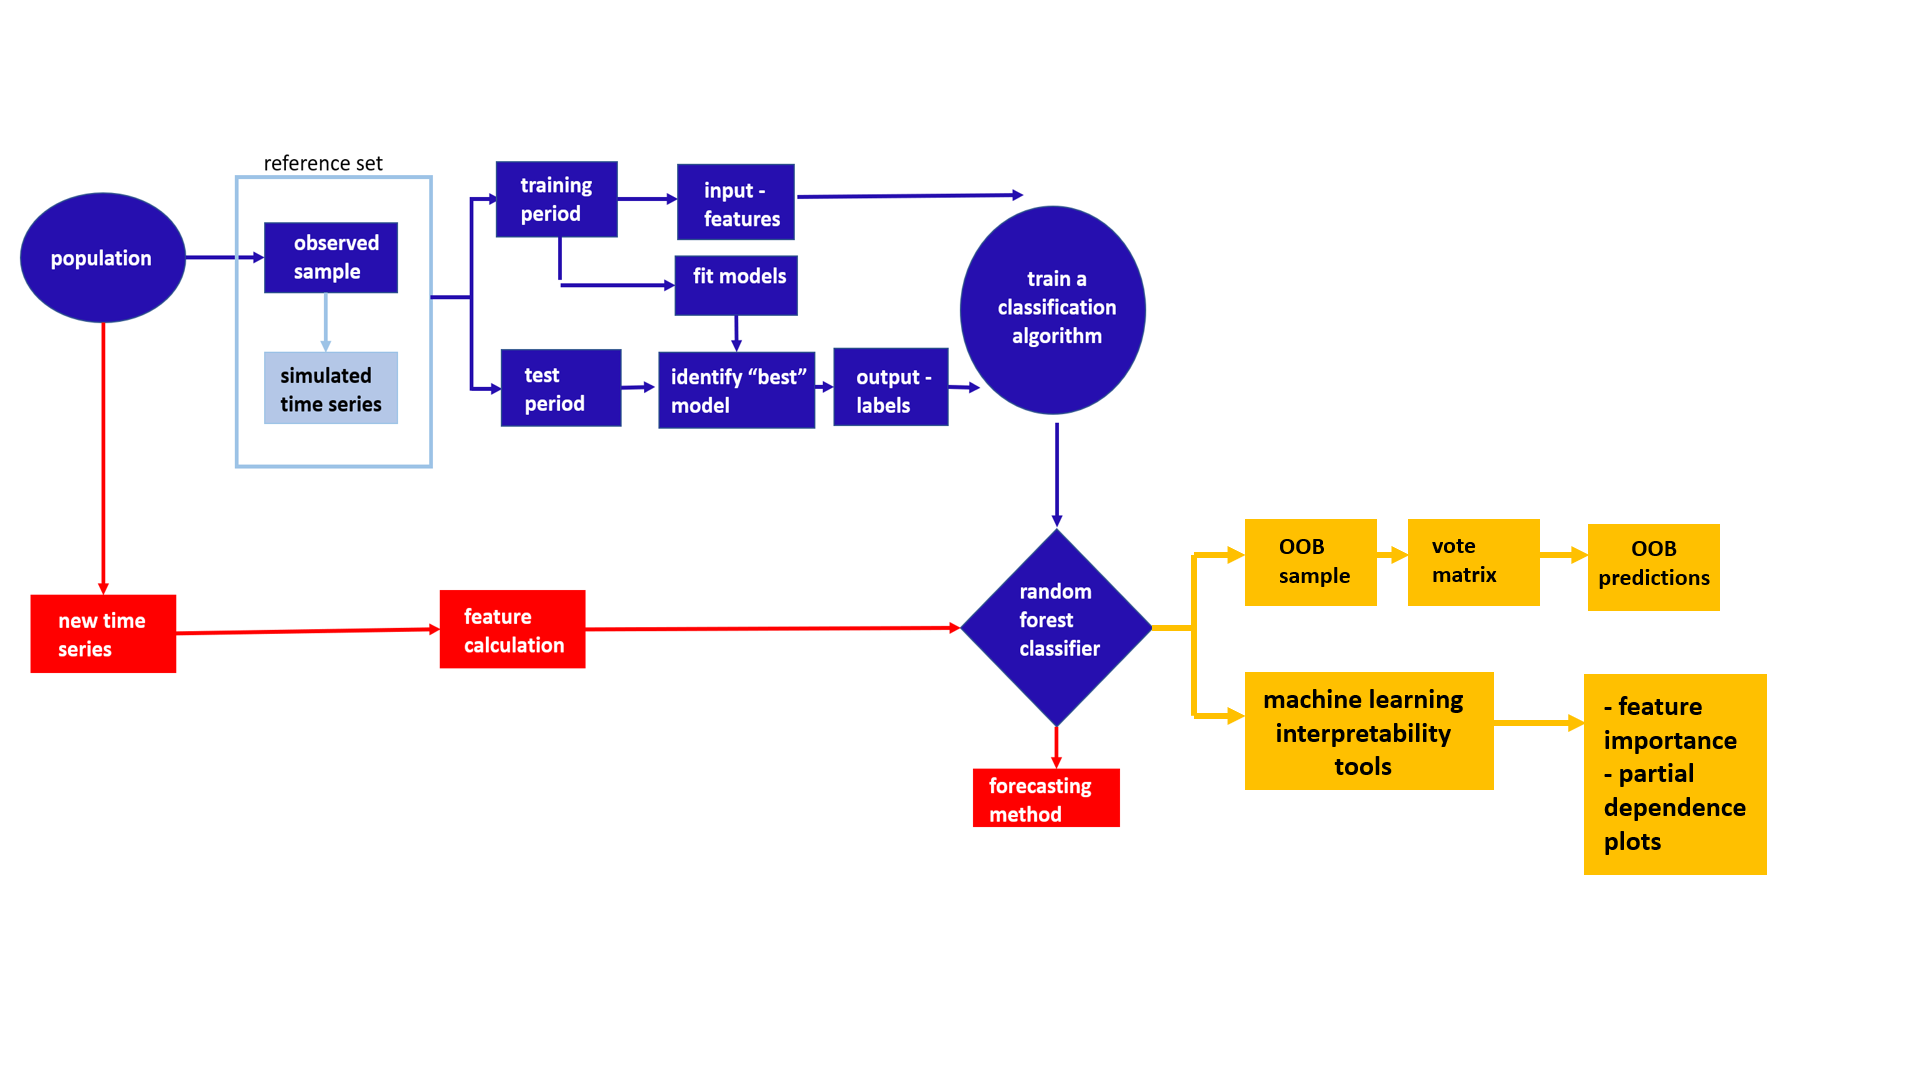
\includegraphics[width=1.15\linewidth]{img/framework2} \caption{extended FFORMS (Feature-based FORecast-Model Selection) framework. The offline phase is shown in blue, the online phase by red and the peeking inside FFORMS is shown in yellow.}\label{fig:framework}
\end{figure}

\hypertarget{offline}{%
\section{Offline phase}\label{offline}}

We now explain application of the FFORMS framework to the M4-competition data. We analyse yearly, quarterly, monthly, weekly, daily and hourly series separately due to their differences in frequencies and hence the appropriateness of different features and forecast-models we considered as class labels.

\hypertarget{reference-set}{%
\subsection{Reference set}\label{reference-set}}

We call the collection of time series used for training the meta-leaner as the ``reference set''. The reference set consist of two sets of time series: i) observed sample and ii) simulated time series.

\hypertarget{observed-sample}{%
\subsubsection{Observed sample}\label{observed-sample}}

We use the time series from the M1, M3 and M4 competitions as the observed sample. Table \ref{observedsample} summarizes the number of time series in the observed sample. Note that from the M4 competition a randomly selected subset of time series are used for the observed sample. The rest shown by the column labelled ``Validation set - M4'' are used as a validation set to evaluate the performance of the meta-learner. Note that, we did not use the test period of the each series of the M4 competition to our observed sample or validation set as it was not available to the competitiors during the running of the M4-competition.

\begin{table}[!h]
\centering
\caption{Composition of the time series in the observed sample and the validation set}
\label{observedsample}
\begin{tabular}{l|rrr|r}
\multirow{2}{*}{Frequency} & \multicolumn{3}{l|}{Observed Sample} & Validation set \\
&   M1    &    M3   &    M4 & M4 \\ \hline
Yearly          &   181    &   645    &   22000 & 1000 \\
Quarterly       &   203    &    756   &   23000 & 1000\\
Monthly         &   617    &    1428   &  47000 & 1000\\
Weekly          &   -    &   -    &   259 & 100\\
Daily           &   -    &   -    &   4001 & 226\\
Hourly          &   -    &    -   &  350 & 64\\ \hline
\end{tabular}
\end{table}

\hypertarget{simulated-time-series}{%
\subsubsection{Simulated time series}\label{simulated-time-series}}

As described in \textcite{fforms}, we augment the reference set by adding multiple time series simulated based on each series in the M4 competition. We use several automated algorithms to simulate multiple time series. The \texttt{ets()} and \texttt{auto.arima()} functions available in the forecast package in R \autocite{forecast} are used to simulate yearly, quarterly and monthly data from exponential smoothing and ARIMA models. The \texttt{stlf()} function also available in the forecast package is used to simulate multiple time series based on multiple seasonal decomposition approach. Using the above functions, we fit models to each time series in the M4 database and then simulate multiple time series from the selected models. In this experiment the length of the simulated time series is set to be equal to: length of the training
period specified in the M4 competition + length of the forecast horizon specified in the competition. For example, the series with id ``Y13190'' contains a training period of length 835. The length of the simulated series generated based on this series is equals to 841 (835+6). Before simulating time series from daily and hourly series, we convert the time series into multiple seasonal time series (msts) objects. For daily time series with length less than 366, the frequency set to 7 and longer time series are converted to multiple seasonal time series objects with frequencies set to 7 and 365.25. For hourly series, we set the frequencies to 24 and 168 to handle multiple frequencies corresponds to time-of-day pattern and time-of-week pattern respectively. We should re-emphasize that all the observed time series and the simulated time series form the reference set to build our meta-learner. Once we create the reference set for random forest training we split each time series in the reference set into training period and test period.

\hypertarget{input-features}{%
\subsection{Input: features}\label{input-features}}

The FFORMS framework operates on features calculated from the time series. For each time series in the reference set, features are calculated based on the training period of the time series.

\begin{table}[!htp]
\centering\footnotesize\tabcolsep=0.12cm
\caption{Time series features}
\label{feature}
\begin{tabular}{llp{8,8cm}cccc}
\toprule
\multicolumn{2}{c}{Feature} & Description & Y & Q/M & W & D/H\\
\midrule
1  & T              & length of time series                                                                   & \yes  & \yes & \yes & \yes\\
2  & trend          & strength of trend                                                                       & \yes  & \yes & \yes & \yes\\
3  & seasonality 1    & strength of seasonality corresponds to frequency 1                                                              & -     & \yes & \yes & \yes\\
4  & seasonality 2    & strength of seasonality corresponds to frequency 2                                                              & -     & - & -& \yes\\
5  & linearity      & linearity                                                                               & \yes  & \yes & \yes & \yes\\
6  & curvature      & curvature                                                                               & \yes  & \yes & \yes & \yes\\
7  & spikiness      & spikiness                                                                               & \yes  & \yes & \yes & \yes\\
8  & e\_acf1        & first ACF value of remainder series                                                     & \yes  & \yes & \yes & \yes\\
9  & stability      & stability                                                                               & \yes  & \yes & \yes & \yes\\
10  & lumpiness      & lumpiness                                                                               & \yes  & \yes & \yes & \yes\\
11 & entropy        & spectral entropy                                                                        & \yes  & \yes & \yes & \yes\\
12 & hurst          & Hurst exponent                                                                          & \yes  & \yes & \yes & \yes\\
13 & nonlinearity   & nonlinearity                                                                            & \yes\ & \yes & \yes & \yes\\
14 & alpha          & ETS(A,A,N) $\hat\alpha$                                                                 & \yes  & \yes & \yes & -\\
15 & beta           & ETS(A,A,N) $\hat\beta$                                                                  & \yes  & \yes & \yes & - \\
16 & hwalpha        & ETS(A,A,A) $\hat\alpha$                                                                 & -     & \yes & - & -\\
17 & hwbeta         & ETS(A,A,A) $\hat\beta$                                                                  & -     & \yes & - & - \\
18 & hwgamma        & ETS(A,A,A) $\hat\gamma$                                                                 & -     & \yes & - &-\\
19 & ur\_pp         & test statistic based on Phillips-Perron test                                            & \yes  & - & - & - \\
20 & ur\_kpss       & test statistic based on KPSS test                                                       & \yes  & - & - & - \\
21 & y\_acf1        & first ACF value of the original series                                                  & \yes  & \yes & \yes & \yes\\
22 & diff1y\_acf1   & first ACF value of the differenced series                                               & \yes  & \yes & \yes & \yes\\
23 & diff2y\_acf1   & first ACF value of the twice-differenced series                                         & \yes  & \yes & \yes & \yes\\
24 & y\_acf5        & sum of squares of first 5 ACF values of original series                                 & \yes  & \yes & \yes & \yes\\
25 & diff1y\_acf5   & sum of squares of first 5 ACF values of differenced series                              & \yes  & \yes & \yes & \yes\\
26 & diff2y\_acf5   & sum of squares of first 5 ACF values of twice-differenced series                        & \yes  & \yes & \yes & \yes \\
27 & sediff\_seacf1 & ACF value at the first seasonal lag of seasonally-differenced series                    & -     & \yes & \yes & \yes\\
28 & sediff\_acf5   & sum of squares of first 5 autocorrelation coefficients of seasonally-differenced series & -     & \yes & \yes & \yes\\
29 & seas\_pacf     & partial autocorrelation coefficient at first seasonal lag & -     & \yes & \yes & \yes\\
30 & lmres\_acf1    & first ACF value of residual series of linear trend model                                & \yes  & - & - & -\\
31 & y\_pacf5       & sum of squares of first 5 PACF values of original series                                & \yes  & \yes & \yes & \yes\\
32 & diff1y\_pacf5  & sum of squares of first 5 PACF values of differenced series                             & \yes  & \yes & \yes & \yes\\
33 & diff2y\_pacf5  & sum of squares of first 5 PACF values of twice-differenced series                       & \yes  & \yes & \yes & \yes\\
\bottomrule
\end{tabular}
\end{table}

The description of the features calculated under each frequency category is shown in Table \ref{feature}. A comprehensive description of the features used in the experiment is given in \textcite{fforms}.

\hypertarget{output-class-labels}{%
\subsection{Output: class-labels}\label{output-class-labels}}

The description of class labels considered under each frequency is shown in Table \ref{classlabels}. Note that these added to \textcite{fforms}. Most of the labels given in Table \ref{classlabels} are self-explanatory labels. In STL-AR, mstlets, and mstlarima, first an STL decomposition is applied to the time series and then seasonal naive is used to forecast the seasonal component. Then, AR, ETS and ARIMA models are used to forecast the seasonally adjusted data respectively. We fit the corresponding models outlined in Table \ref{classlabels} to each series in the reference set. The models are estimated using the training period for each series, and forecasts are produced for the test periods.

\begin{table}[!htp]
\centering\footnotesize\tabcolsep=0.12cm
\caption{Class labels}
\label{classlabels}
\begin{tabular}{llrrrr}
class label & Description & Y & Q/M & W & D/H \\ \hline
WN & white noise process & \checkmark & \checkmark & \checkmark & \checkmark \\
AR/MA/ARMA & AR, MA, ARMA processes & \checkmark & \checkmark & \checkmark & -\\
ARIMA & ARIMA process & \checkmark & \checkmark & \checkmark & - \\
SARIMA & seasonal ARIMA & \checkmark & \checkmark & \checkmark & -\\
RWD & random walk with drift & \checkmark & \checkmark & \checkmark & \checkmark \\
RW & random walk & \checkmark & \checkmark & \checkmark & \checkmark  \\
Theta & standard theta method & \checkmark & \checkmark & \checkmark & \checkmark \\
STL-AR &  & - & \checkmark & \checkmark & \checkmark \\
ETS-notrendnoseasonal & ETS without trend and seasonal components & \checkmark & \checkmark & \checkmark & - \\
ETStrendonly & ETS with trend component and without seasonal component & \checkmark & \checkmark & \checkmark & -\\
ETSdampedtrend & ETS with damped trend component and without seasonal component  & \checkmark &  \checkmark & - & - \\
ETStrendseasonal & ETS with trend and seasonal components & - & \checkmark & - & - \\
ETSdampedtrendseasonal & ETS with damped trend and seasonal components & - & \checkmark & - & -\\
ETSseasonalonly & ETS with seasonal components and without trend component & -  & \checkmark & - & - \\
snaive & seasonal naive method & \checkmark & \checkmark & \checkmark & \checkmark \\
tbats & TBATS forecasting & - & \checkmark & \checkmark & \checkmark \\
nn & neural network time series forecasts & \checkmark & \checkmark & \checkmark & \checkmark \\
mstlets &  & - & - & \checkmark & \checkmark \\
mstlarima & & - & - & - & \checkmark \\\hline
\end{tabular}
\end{table}

According to the \textcite{M4compguide}, in the M4-competition the forecast accuracy is evaluated based on the mean Absolute Scaled Error (MASE) and the symmetric Mean Absolute Percentage Error (MAPE). Hence, in order to identify the ``best'' forecast-model for each time series in the reference set we combine MASE and the symmetric MAPE calculated over the test set. More specifically, for each series both forecast error measures MASE and sMAPE are calculated for each of the forecast models. Each of these is respectively standardized by the median MASE and median sMAPE calculated across the forecast-models. The model with the lowest average value of the scaled MASE and scaled sMAPE is selected as the output class-label.

The last step of offline phase of the framewok is to train a meta-learner. A random forest algorithm is used to train the meta-learner.

\hypertarget{online}{%
\section{Online phase}\label{online}}

The online phase of the algorithm involves generating point forecasts and 95\% prediction intervals for the new series or the future values observed time series. We calculate point forecasts and prediction intervals over the test period of M4-competition data. First, the corresponding features are calculated based on the full length of the training period provided by the M4 competition. Second, point forecasts and 95\% prediction intervals are calculated based on the predicted class labels. We should note that all negative forecasts are set to zero.

\hypertarget{peeking}{%
\section{Peeking inside FFORMS}\label{peeking}}

The main objective of this paper is to explore the nature of the relationship between features and forecast-model selection learned by the FFORMS framework. More specifically, to identify which of the features are important for model predictions and how different features and their interactions led to the different choices. First, we explore the global role of features in the choice of different forecast-model selection. Global interpretability evaluates the behavior of a model on entire data set. Global perspective of model interpretation helps users to understand the overall modeled relationship between features and the FFORMS outcome. In the following subsections, we provide a description of tools we use to explore the global perspective of the FFORMS meta-learners.

\hypertarget{visualise-patterns-learned-by-the-meta-learner}{%
\subsection{Visualise patterns learned by the meta-learner}\label{visualise-patterns-learned-by-the-meta-learner}}

A useful by-product of random forest is Out-Of-Bag (OOB) observations. The observations not included in building a given tree is called OOB observations. In general, each bagged tree does not make use of around one third of observations to construct a tree. Furthermore, each tree is grown based on different bootstrap samples hence, each tree has different set of OOB observations. We use a vote matrix calculated based on OOB observations to visualise patterns leaned by the random forest. The vote matrix (\(N \times P\); \(N\) is total number of observations, \(P\) is number of classes) contains the proportion of times each observation was classified to each class based on OOB observations.

\hypertarget{feature-importance}{%
\subsection{Feature importance}\label{feature-importance}}

\textcite{jiang2002} explains variable importance under three different views: i) causality: change in the value of Y for an increase or decrease in the value of x, ii) contribution of X based on out-of-sample prediction accuracy and iii) face value of X on prediction function \(g\), for example in linear regression model estimated coefficients of each predictor can be considered as a measure of variable importance. See \textcite{jiang2002} for comparable face value interpretation for machine learning models. In this paper we use the first two notions of variable importance. Partial dependency functions and individual conditional expectation curves are used to explore the ``causality'' notion of variable importance while Mean decrease in Gini coefficient and Permutation-based variable importance are used to capture the second notion of variable importance-features contribution to the predictive accuracy (\textcite{Zhao}). We will introduce each of these variable importance measures below.

Let \(\mathcal{P}=\{(\mathbf{x^{(i)}}, y^{(i)})\}_{i=1}^{N}\) be the
historical data set we use to train a classifier. Consider a
p-dimensional feature vector \(X=(X_1, X_2, ..., X_p)\) and a dependent
variable, the best forecasting method for each series \(Y\). Let \(\mathcal{G}\) be the unknown relationship between \(X\) and
\(Y\). \textcite{Zhao} term this as ``law of nature''. Inside the FFORMS framework, random forest algorithm tries to learn this relationship using
the historical data we provided. We denote the predicted function as
\(g\).

\hypertarget{mean-decrease-in-gini-coefficient}{%
\subsubsection{Mean decrease in Gini coefficient}\label{mean-decrease-in-gini-coefficient}}

Mean decrease in Gini coefficient is a measure of how each feature contributes to the homogeneity of the nodes and leaves in the resulting random forest proposed by \textcite{breiman2001random}.

\hypertarget{permutation-based-variable-importance-measure}{%
\subsubsection{Permutation-based variable importance measure}\label{permutation-based-variable-importance-measure}}

The permutation-based variable importance introduced by \textcite{breiman2001random} measures the prediction
strength of each feature. This measure is calculated based on the out-of-bag (OOB) observations. The calculation of variable importance is formalized as follow: Let \(\bar{\mathcal{B}}^{(k)}\) be the OOB sample for a tree \(k\), with \(k\in \{1,...,ntree\}\), where \(ntree\) is the number of trees in the random forest. Then the variable importance of variable \(X_{j}\) in \(k^{th}\) tree is:
\[VI^{(k)}(X_{j})=\frac{\sum_{i\in \bar{\mathcal{B}}^{(k)}}I(\gamma_{i}=\gamma_{i,\pi_{j}}^{k})}{|\bar{\mathcal{B}}^{(k)}|}-\frac{\sum_{i\in \bar{\mathcal{B}}^{(k)}}I(\gamma_{i}=\gamma_{i}^{k})}{|\bar{\mathcal{B}}^{(k)}|},\]
where \(\gamma_{i}^{k}\) denotes the predicted class for the \(i^{th}\) observation before permuting the values of \(X_{j}\) and \(\gamma_{i, \pi_{j}}^{k}\) is the predicted class for the \(i^{th}\) observation after permuting the values of \(X_{j}\). The overall variable importance score is calculated as:
\[VI(X_{j})=\frac{\sum_{1}^{ntree}VI^{(t)}(x_{j})}{ntree}.\]

Permutation-based variable importance measures provide a useful starting point for identifying relative influence of features on the predicted outcome. However, they provide a little indication of the nature of the relationship between the features and model outcome. To gain further insights into the role of features inside the FFORMS framework we use partial dependence plot (PDP) introduced by \textcite{friedman2008predictive}.

\hypertarget{partial-dependence-plot-pdp-and-variable-importance-measure-based-on-pdp}{%
\subsubsection{Partial dependence plot (PDP) and Variable importance measure based on PDP}\label{partial-dependence-plot-pdp-and-variable-importance-measure-based-on-pdp}}

Partial dependence plot can be used to graphically examine how each feature is related to the model prediction while accounting for the average effect of other features in the model. Let \(X_s\) be the subset of features we want examine partial dependencies for and \(X_c\) be the remaining set of features in \(X\). Then \(g_s\), the partial dependence function on \(X_s\) is defines as
\[g_s(X_s)=E_{x_c}[g(x_s, X_c)]=\int{g(x_s, x_c)dP(x_c).}\]
In practice, PDP can be estimated from a training data set as
\[\bar{g_s}(x_s)=\frac{1}{n}\sum_{i=1}^{n}g(x_s, X_{iC}),\]
where \(n\) is the number of observations in the training data set. Partial dependency curve can be created by plotting the pairs of \(\{(x_s^k, \bar{g}_s(x_{sk}))\}_{k=1}^{m}\) defined on grid of points \(\{x_{s1}, x_{s2},\dots, x_{sm}\}\) based on \(X_s\). FFORMS framework has treated the forecast-model selection problem as a classification problem. Hence, in this paper partial dependency functions display the probability of certain class occurring given different values of the feature \(X_s\).

\textcite{Greenwell2018} introduce a variable importance measure based on the partial dependency curves. The idea is to measure the ``flatness'' of partial dependence curves for each feature. A feature whose PDP curve is flat, relative to the other features, indicates that the feature does not have much influence on the predicted value as it changes while taking into account the average effect of the other features in the model. The flatness of the curve is measured using the standard deviation of the values \(\{\bar{g}_{s}(x_{sk})\}_{k=1}^{m}\).

\hypertarget{individual-conditional-expectation-ice-curves-variable-importance-measure-based-on-ice-curves}{%
\subsubsection{Individual conditional expectation (ICE) curves Variable importance measure based on ICE curves}\label{individual-conditional-expectation-ice-curves-variable-importance-measure-based-on-ice-curves}}

While partial dependency curves are useful in understanding the estimated relationship between features and the predicted outcome in the presence of substantial interaction between features, it can be misleading. \textcite{goldstein2015peeking} propose the Individual Conditional Expectation (ICE) curves to address this issue. Instead of
averaging \(g(x_s, X_{iC})\) over all observations in the training data, ICE plots the individual response curves by plotting the pairs \(\{(x_s^k, g(x_{sk}, X_{iC}))\}_{k=1}^{m}\) defined on grid of points \(\{x_{s1}, x_{s2},\dots, x_{sm}\}\) based on \(X_s\). In other words, partial dependency curve is simply the average of all the ICE curves.

This method is similar to the PDP-based variable importance scores above, but are based on measuring the ``flatness'' of the individual conditional expectation curves. We calculated standard deviations of each ICE curves. We then computed an ICE based variable importance score -- simply the average of all the standard deviations. A higher value indicates a higher degree of interactivity with other features.

\hypertarget{ranking-of-features-based-on-feature-importance-measures}{%
\subsubsection{Ranking of features based on feature importance measures}\label{ranking-of-features-based-on-feature-importance-measures}}

To identify class-specific important features we rank features in three different ways: i) based on permutation-based variable importance, ii) based on partial dependence functions and iii) based on ICE-curves. We consider 25 features for yearly data. The feature that shows the highest importance is ranked 25, the second best is ranked 24, and so on. Finally, for each feature, a mean rank is calculated based on the rankings of the three measures. Similarly, the overall feature importance is evaluated based on the permutation-based variable importance measure and the Gini coefficient-based feature importance measure.

\hypertarget{relationship-between-most-important-features-and-the-choice-of-forecast-model-selection}{%
\subsection{Relationship between most important features and the choice of forecast-model selection}\label{relationship-between-most-important-features-and-the-choice-of-forecast-model-selection}}

The partial-dependence curves along with their confidence intervals are used to visualize the relationship between top features are the choice of forecast model selection.

\hypertarget{assessment-of-interaction-effect}{%
\subsection{Assessment of interaction effect}\label{assessment-of-interaction-effect}}

Friedman's H-statistic (\textcite{friedman2008predictive}) is used to test the presence of interaction between all possible pairs of features. This statistic is computed based on the partial dependence functions. For two-way interaction between two specific variable \(x_j\) and \(x_k\), Friedman's H-statistic is defined as follow,

\[H_{jk}^2=\sum_{i=1}^{n}[\bar{g}_{s}(x_{ij}, x_{jk})-\bar{g}_{s}(x_{ij})-\bar{g}_{s}(x_{ik})]^2/\sum_{i=1}^{n}\bar{g}^2_{s}(x_{ij}, x_{jk}).\]

The Friedman's H-statistic measures the fraction of variance of two-variable partial dependency, \(\bar{g}_{s}(x_{ij}, x_{jk})\) not captured by sum of the respective individual partial dependencies, \(\bar{g}_{s}(x_{ij})+\bar{g}_{s}(x_{ik})\). In addition to Friedman's H-statistic we also use the PDP of two variables to visualize the interaction effects.

Note that the, PD plots, ICE curves and PD-, ICE-associated measures and Friedman's H-statistic are computationally intensive to compute, especially when there are large number of observations in the training set. Hence, in our experiments ICE and PDP-based variable importance measures are computed based on the subset of randomly selected training examples.

\hypertarget{local-interpretable-model-agnostic-explanations-lime}{%
\subsection{Local Interpretable Model-agnostic Explanations (LIME)}\label{local-interpretable-model-agnostic-explanations-lime}}

Global interpretations help us to understand the entire modelled relationship. Local interpretations help us to understand the predictions of the model for a single instance or a group of similar instances. In other words, this allows users to zoom into a particular instance or a subset and explore how different features affect the resulting prediction. We use Local Interpretable Model-agnostic Explanations (LIME) approach introduce by \textcite{ribeiro2016should} for explaining individual predictions which relies on the assumption that ``every complex model is linear on a local scale''. This is accomplished by locally approximating the complex black-box model with a simple interpretable model. \textcite{ribeiro2016should} highlighted features that are globally important may not be important in the local context and vice versa. The algorithm steps can be summarized as follow:

\begin{enumerate}
\def\labelenumi{\arabic{enumi}.}
\tightlist
\item
  Select an observation of interest which we need to have explanations for its black-box prediction.
\item
  Create a permuted data set based on the selected observation. Permuted data set is created by making slight modifications to the features of selected observations.
\item
  Obtain similarity scores by calculating distance between permuted data and selected observation.
\item
  Obtain predicted outcomes for all permuted data using the black-box model.
\item
  Select \(m\) number of features best describing the black-box model outcome. This can be accomplished by applying feature selection algorithms such as ridge regression, lasso, etc.
\item
  Fit a simple linear model to the permuted data based on \(m\) selected features, similarity scores in step 3 as weights and complex model prediction outcomes in step 4 as response variable.
\item
  Use the estimated coefficients of simple linear model to explain the local behaviour corresponds to the selected observation in step 1.
\end{enumerate}

An alternative for explaining local behaviour of complex models is proposed by \textcite{lundberg2017unified} based on game theory named ``Shapley values''.

\hypertarget{results1}{%
\section{Evaluation based on the M4 competition data}\label{results1}}

\autoref{forecasts} shows the performance of FFORMS approach on the M4 competition data. The point forecasts and prediction intervals are evaluated based on the test period of each series. The point forecasts are evaluated based on MASE computed for each forecast horizon, and then by averaging the MASE errors across all series corresponds to each frequency category. Similarly, MSIS is used to evaluate the prediction intervals. The results are compared against several bench marks and top three (3) winners of the M4 competition. The top ranking methods of M4 competition are based on some kind of combination approach. The 1st ranking method is based on hybrid approach which produce forecasts based on both ETS and Machine-Learning approach. The 2nd and 3rd places were based on combination of seven-eight different forecast-models. The 2nd and 3rd approaches are time consuming because forecasts from all candidate models must be computed. The results of FFORMS approach is based on individual forecasts. According to the \autoref{forecasts}, we can see FFORMS approach achieved comparable performance in much more cost-effective and time-effective way. Based on FFORMS approach we provided an entry to the M4 competition. After submission we found a bug in our implementation for hourly data, hence only for hourly data results are different with the published results of the M4 competition. Results of yearly, quarterly, monthly, weekly and daily data are same as the published results. This completes the evaluation of FFORMS framework. The main question we have now is ``Can we trust the FFORMS framework if we do not know how it works?'' In the next section we present results of what is happening inside the FFORMS framework?

\begin{table}[!h]
\centering\scriptsize\tabcolsep=0.12cm
\caption{The performance of FFORMS on the M4 competition data based on point forecasts (based on MASE) and prediction intervals (based on MSIS)}
\label{forecasts}
\begin{tabular}{l|rrrrrr}
\hline
\multicolumn{7}{c}{Point Forecasts (Mean Absolute Scaled Error (MASE))} \\\hline
 & Yearly & Quarterly & Monthly & Weekly & Daily & Hourly \\\hline
\bf{FFORMS} & \bf{3.17} &  \bf{1.20} &  \bf{0.98}&  \bf{2.31}& \bf{3.57} &  \bf{0.84}\\
auto.arima & 3.40 &1.17  &0.93  & 2.55 &  -& - \\
ets & 3.44 &  1.16& 0.95 &  -&-  &  -\\
theta & 3.37 &1.24  & 0.97 &2.64  & 3.33 & 1.59 \\
rwd & 3.07 & 1.33 & 1.18  & 2.68  & 3.25 & 11.45 \\
rw & 3.97 & 1.48 & 1.21  &2.78  & 3.27 & 11.60 \\
nn & 4.06 & 1.55 &  1.14 &4.04 & 3.90 & 1.09 \\
stlar & - & 2.02 &  1.33& 3.15 & 4.49 & 1.49 \\
snaive & - &  1.66& 1.26 &  2.78& 24.46 & 2.86 \\
tbats & - & 1.19 &  1.05& 2.49 & 3.27 &  1.30\\
wn & 13.42 &  6.50&  4.11&  49.91& 38.07 & 11.68 \\
mstlarima & - & - &  - & - & 3.84 &  1.12\\
mstlets & - &  - &  - &  - & 3.73 &  1.23\\
combination (mean) & 4.09 & 1.58 &  1.16&6.96  & 7.94 & 3.93 \\\hline
M4-1st & 2.98 & 1.12 &  0.88& 2.36 & 3.45 & 0.89\\
M4-2nd & 3.06 & 1.11 &  0.89& 2.11 & 3.34 & 0.81\\
M4-3rd & 3.13 & 1.23 &  0.95& 2.16 & 2.64 & 0.87\\\hline
\multicolumn{7}{c}{Prediction Intervals (Mean Scaled Interval Score (MSIS))} \\\hline
\bf{FFORMS} & \bf{39.79} &  \bf{11.24} &  \bf{9.82}&  \bf{20.84}& \bf{36.36} &  \\
M4-1st & 23.89 & 8.55 &  7.20 & 22.03 & 26.28 & 7.92\\
M4-2nd & 27.47 & 9.38 &  8.65& 21.53 & 34.37 & 18.50\\
M4-3rd & \multicolumn{6}{c}{not submitted}\\\hline
\end{tabular}
\end{table}

\hypertarget{results2}{%
\section{What is happening under the hood of FFORMS?}\label{results2}}

\hypertarget{yearly-series}{%
\subsection{Yearly series}\label{yearly-series}}

This vote-matrix information for the yearly data is presented in \autoref{fig:yearlyoob}. \autoref{fig:yearlyoob} indicates three primary patterns: i) the distributions of correctly classified classes dominate, indicating a good classification of the meta-learner, the associated outliers of the boxplots indicate some series are correctly classified with high probability ii) irrespective of the class labels the random walk with drift has a high chance of getting selected for all series,
(the results if \autoref{results1} also show random walk with drift give very high prediction accuracy with yearly series), iii) FFORMS framework successfully learned the similarities and dissimilarities between the classes itself. For example, within ETS models with a trend component (ETS\_T, 3rd panel), disparities between forecast-models with trend components and forecast-models without trend component (wn, ARMA, ETS\_NTNS) are immediately visible.

\begin{figure}
\centering
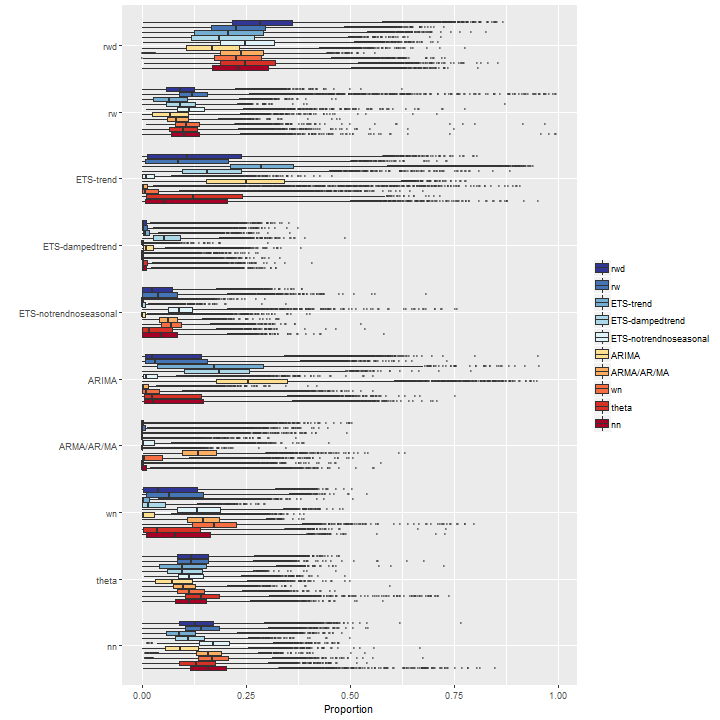
\includegraphics{figures/yearlyoob-1.png}
\caption{\label{fig:yearlyoob}Visualization of the vote matrix based on OOB sample for yearly random forest. Each panel shows the predicted class from the random forest. The X-axis denotes the proportion of times each time series was classified to each class. The colours of boxplots correspond to class label of the ``best'' forecast-model identified based on MASE and sMAPE. On each row, distribution of correctly classified class dominates, indicating a good classification of the meta-learner.}
\end{figure}

\autoref{fig:viyearly} shows how important each one of the features we considered in the overall classification mechanism of the FFORMS as well as within each class. The first panel gives the ranks of overall variable importance for all features and the other panels shows the class-specific feature rankings. The main point here is strength of trend and test statistic based on Phillips-Perron unit root test, first ACF value of the differenced series, and linearity are the most important features across all categories.
In addition to that within first ACF value of residual series of linear trend model appear to be important within all classes. In addition to linearity, the other features related to different types of trend (damped trend: measured by \texttt{beta}, exponential trend: measured by curvature) are assigned a very high importance with in ETS\_T, ETS\_DT and ETS\_NTNS which handles different versions of trend within ETS family. Spikiness appear to be an important feature in the overall classification, even though it does not appear to be among top five feature, spikiness has been assigned a relatively high importance within all categories. The reason for the high importance of spikiness within overall classification is due to the high Mean Decrease in Gini Coefficient. This suggests contribution of spikiness to the homogeneity of the nodes and leaves in the resulting random forest make it important rather than its effect of causality. The length of time series (N) is assigned a very low importance within all categories.

\begin{figure}
\centering
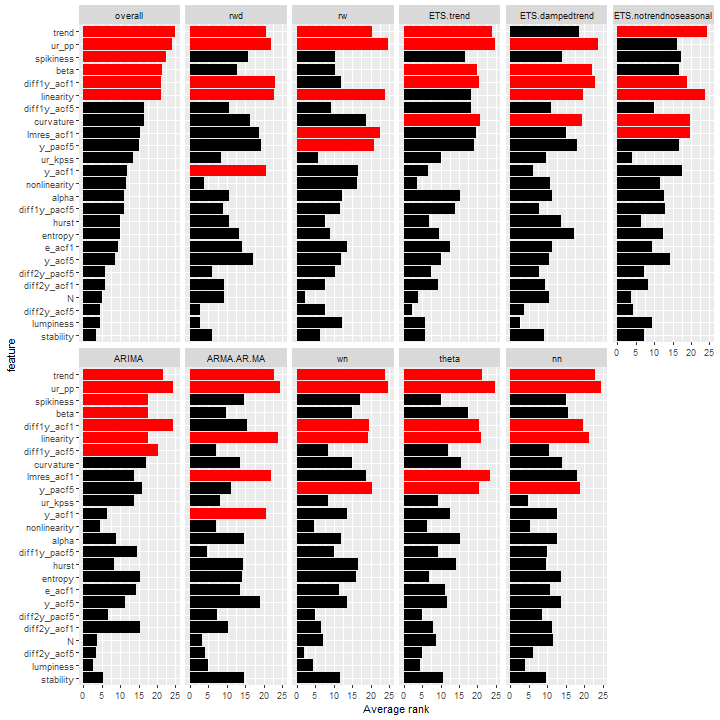
\includegraphics{figures/viyearly-1.pdf}
\caption{\label{fig:viyearly}Feature importance plot for yearly series. Overall feature importance(top left plot) is evaluated based on two measures: i) Permutation-based variable importance measure and ii) mean decrease in Gini coefficients. Class-specific feature importance is evaluated based on three measures: i) permutation-based variable importance, PD-based variable importance measure, and ICE-based variable importance measure. Longer bars indicate more important features. Top 5 overall features are highlighted in purple. Strength of trend appears to be the most important feature.}
\end{figure}

\autoref{fig:pdpyearlyurpp} to \autoref{fig:pdpyearlylinearity} show the partial dependency curves, and associated confidence intervals of the top-three features that get selected most and top within each class. In all three cases, within each class the displayed relationship consistent with the theoretical expectations. For example, a high negative value of Phillips-Perron test statistic indicate a stationarity of the series while a positive value of the test statistic indicate nonstationarity of the series. According to \autoref{fig:pdpyearlyurpp} we can see probability of selecting ETS model with trend component and ARIMA models increases steadily as ur\_pp increases while the opposite relationship could be observed for ARMA and WN. According to \autoref{fig:pdpyearlytrend} we can see the information about whether the strength of trend in the series is extremely high or not matters a lot in selecting a forecast-model. The probability of selecting ETS model without trend components (ETS\_NTNS), WN and ARMA decreases when the strength of trend is extremely high while the opposite relationship could be observed for other classes.

\begin{figure}
\centering
\includegraphics{figures/pdpyearlyurpp-1.pdf}
\caption{\label{fig:pdpyearlyurpp}Partial dependence plots for ur\_pp.~The shading shows the 95\% confidence intervals. Y-axis denotes the probability of belong to corresponding class. All classes show a turning point in the relationship around zero.}
\end{figure}

\begin{figure}
\centering
\includegraphics{figures/pdpyearlytrend-1.pdf}
\caption{\label{fig:pdpyearlytrend}Partial dependence plots for trend. The shading shows the 95\% confidence intervals. Y-axis denotes the probability of belong to corresponding class. Probability of selecting ETS models without a trend component and stationary models (WN and ARMA) decrease for an extremely high value of trend.}
\end{figure}

\begin{figure}
\centering
\includegraphics{figures/pdpyearlylinearity-1.png}
\caption{\label{fig:pdpyearlylinearity}Partial dependence plots for linearity. The shading shows the 95\% confidence intervals. Y-axis denotes the probability of belong to corresponding class. Random walk with drift and ARMA classes are highly sensitive to the value of linearity aound 0.}
\end{figure}

\begin{figure}
\centering
\includegraphics{figures/intyearly-1.png}
\caption{\label{fig:intyearly}Partial dependence plot of model selection probability and the interaction of linearity and diff1y\_acf1 for yearly data. Dark regions show the high probability of belonging to the corresponding class shown in the plot title. Random walk and random walk with drift class show opposite pattern of interactivity between sediff\_seacf1 and linearity.}
\end{figure}

\hypertarget{quarterly-series}{%
\subsection{Quarterly series}\label{quarterly-series}}

\autoref{fig:oobquarterly} shows the vote-matrix of the random forests for quarterly based on OOB observations. The disparities between dominating class and non-dominating classes are immediately apparent within ETS\_DT, ETS\_T, ETS\_DTS, ETS\_TS, ETS\_S and ARMA classes. Within each panel, the outliers associated with dominating distribution indicate some series are correctly classified with very high probability. Furthermore, except ETS\_DTS, ETS\_TS, ETS\_S and SARIMA all other series has a high chance of classified into random walk with drift class. Within the theta, and nn all distributions level at similar proportionalities as they both represent a general class of forecast-models. Overall random forest successfully learnt the similarities and dissimailarities between different forecast-models. For example, within each panel, series with a label which involves a seasonal parameter have a high chance of getting selected a seasonal forecast models such as SARIMA, ETS models with seasonal components, stlar, and tbats.

\autoref{fig:viquarterly} shows the feature importance plots for the quarterly. The features strength of seasonality, trend,diff1y\_pacf5, linearity and spikiness are the most important features across all categories. Even though the lumpiness does not appear as a top five feature within classes it is appeared to be an important feature in the overall classification process and a relatively high ranks are assigned within many classes. Except, ETS\_DT, ETS\_DTS and ETS\_TS the features, nonlinearity, hwalpha and hwbeta are assigned a very low importance within all other classes.

\begin{figure}
\centering
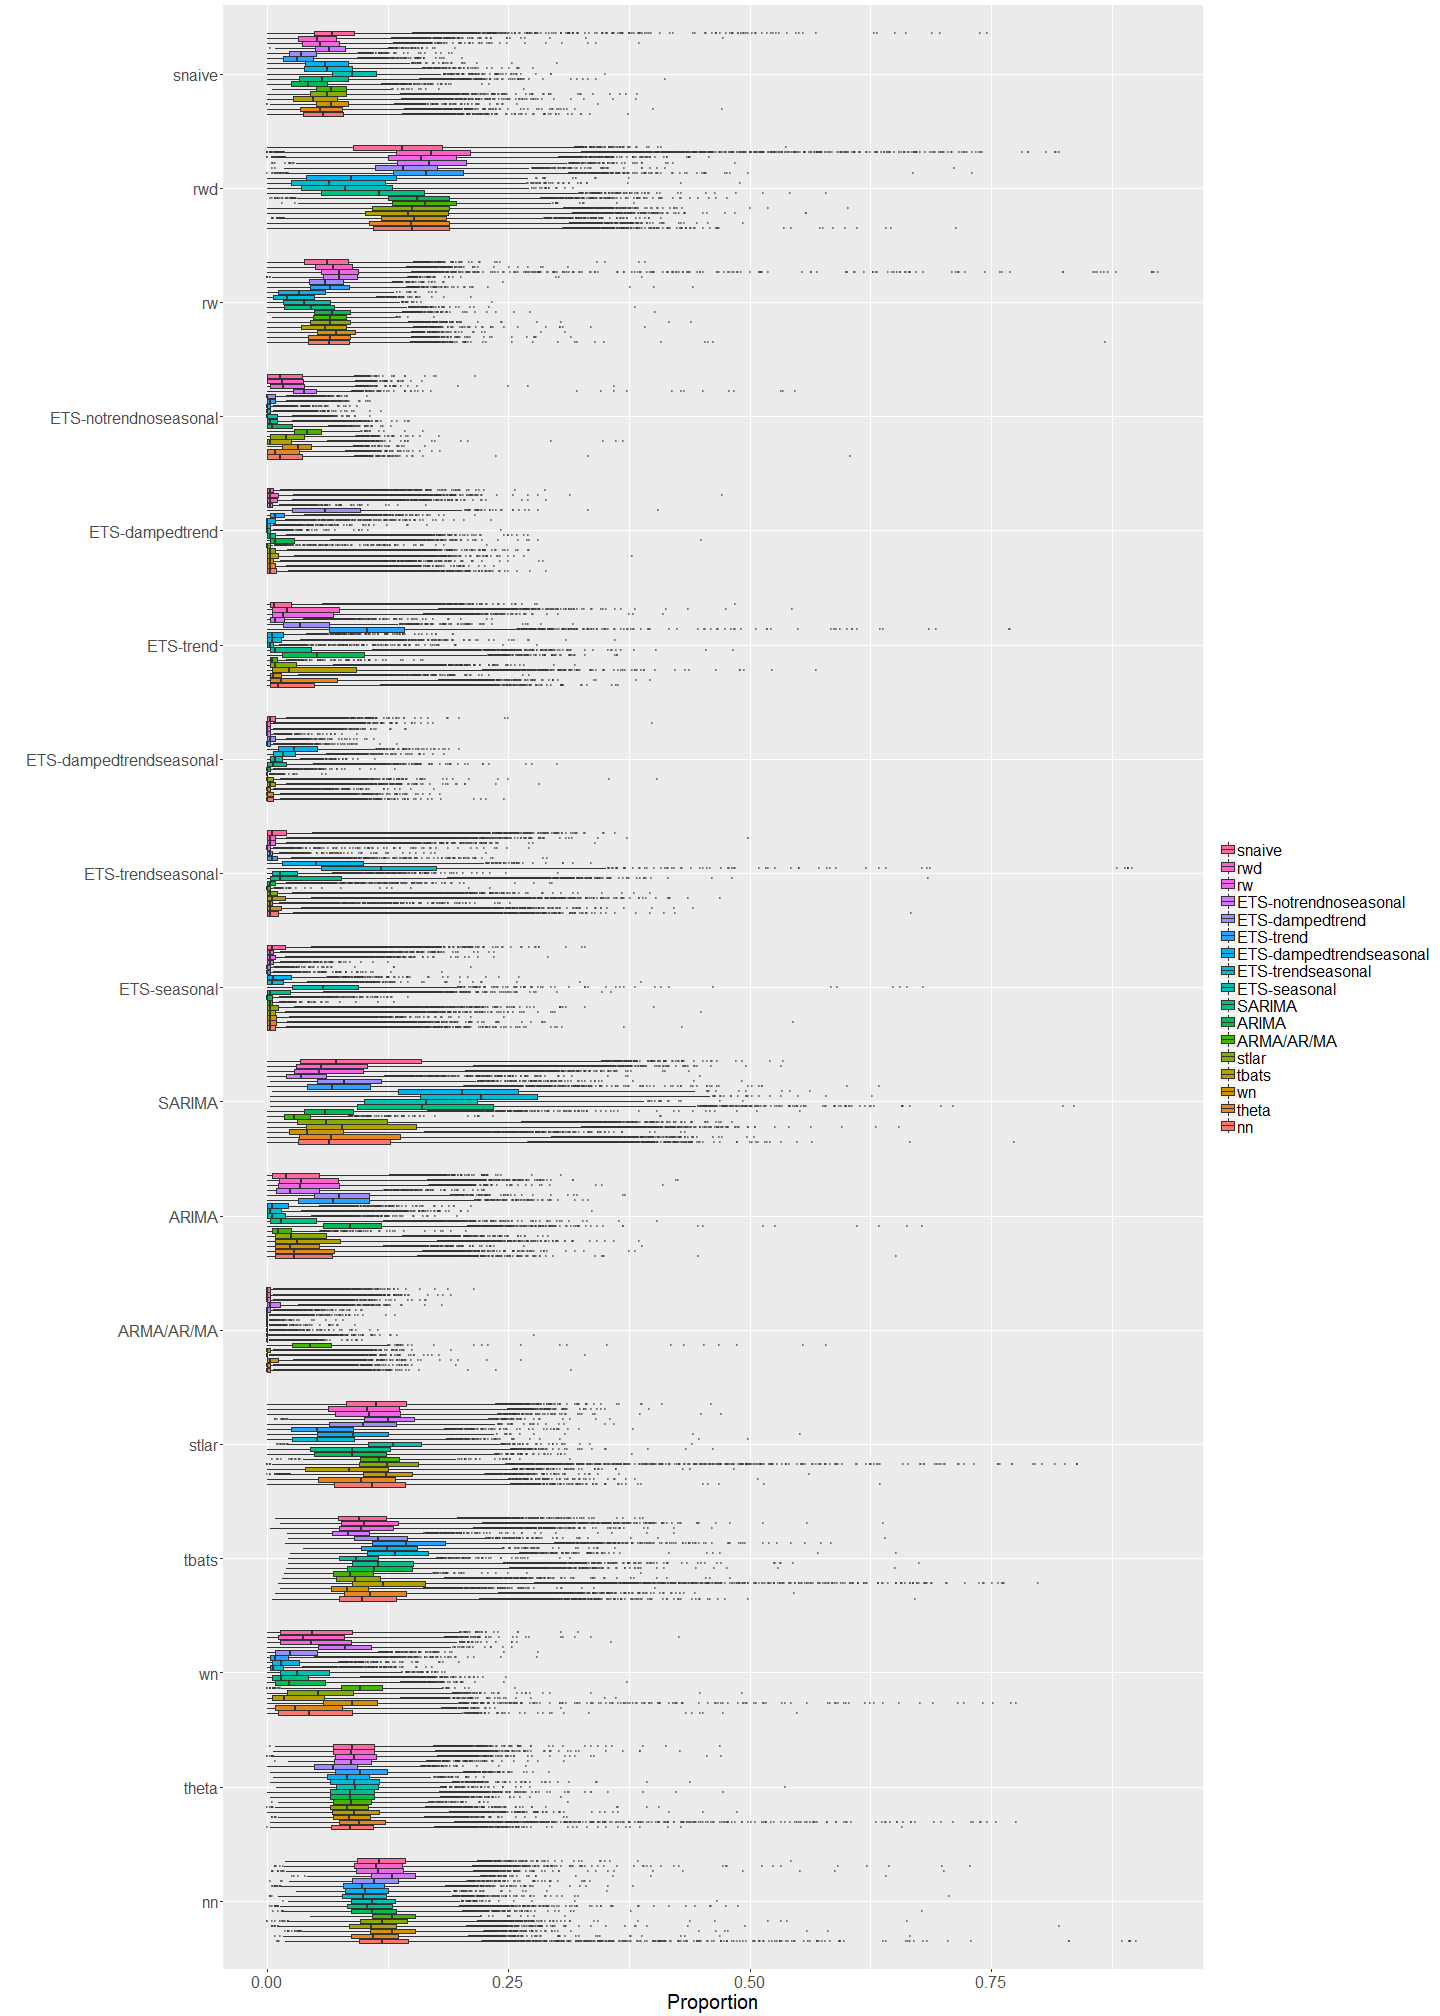
\includegraphics{figures/oobquarterly-1.png}
\caption{\label{fig:oobquarterly}Visualization of the vote matrix based on OOB sample for quarterly random forest. Each panel shows the predicted class from the random forest. The X-axis denotes the proportion of times each time series was classified to each class. The colours of boxplots correspond to class label of the ``best'' forecast-model identified based on MASE and sMAPE. The disparities between dominating class and nondominating classes are immediately apparent within ETS model classes.}
\end{figure}

\autoref{fig:pdpquarterlyseasonality} to \autoref{fig:pdpquarterlytrend} show the partial dependency curves, and associated confidence intervals of the top-three features that get selected most in each class. According to \autoref{fig:pdpquarterlyseasonality}, it is immediately apparent, that the probability of selecting a seasonal forecast-model increases as the strength of seasonality increases. According to \autoref{fig:pdpquarterlyseasonality} and \autoref{fig:pdpquarterlydiff1ypacf5} probability of selecting SARIMA models drastically changes according to the change of seasonality, and diff1y\_pacf5. The partial dependence plot of trend is very similar to the observed patterns in yearly data.

\begin{figure}
\centering
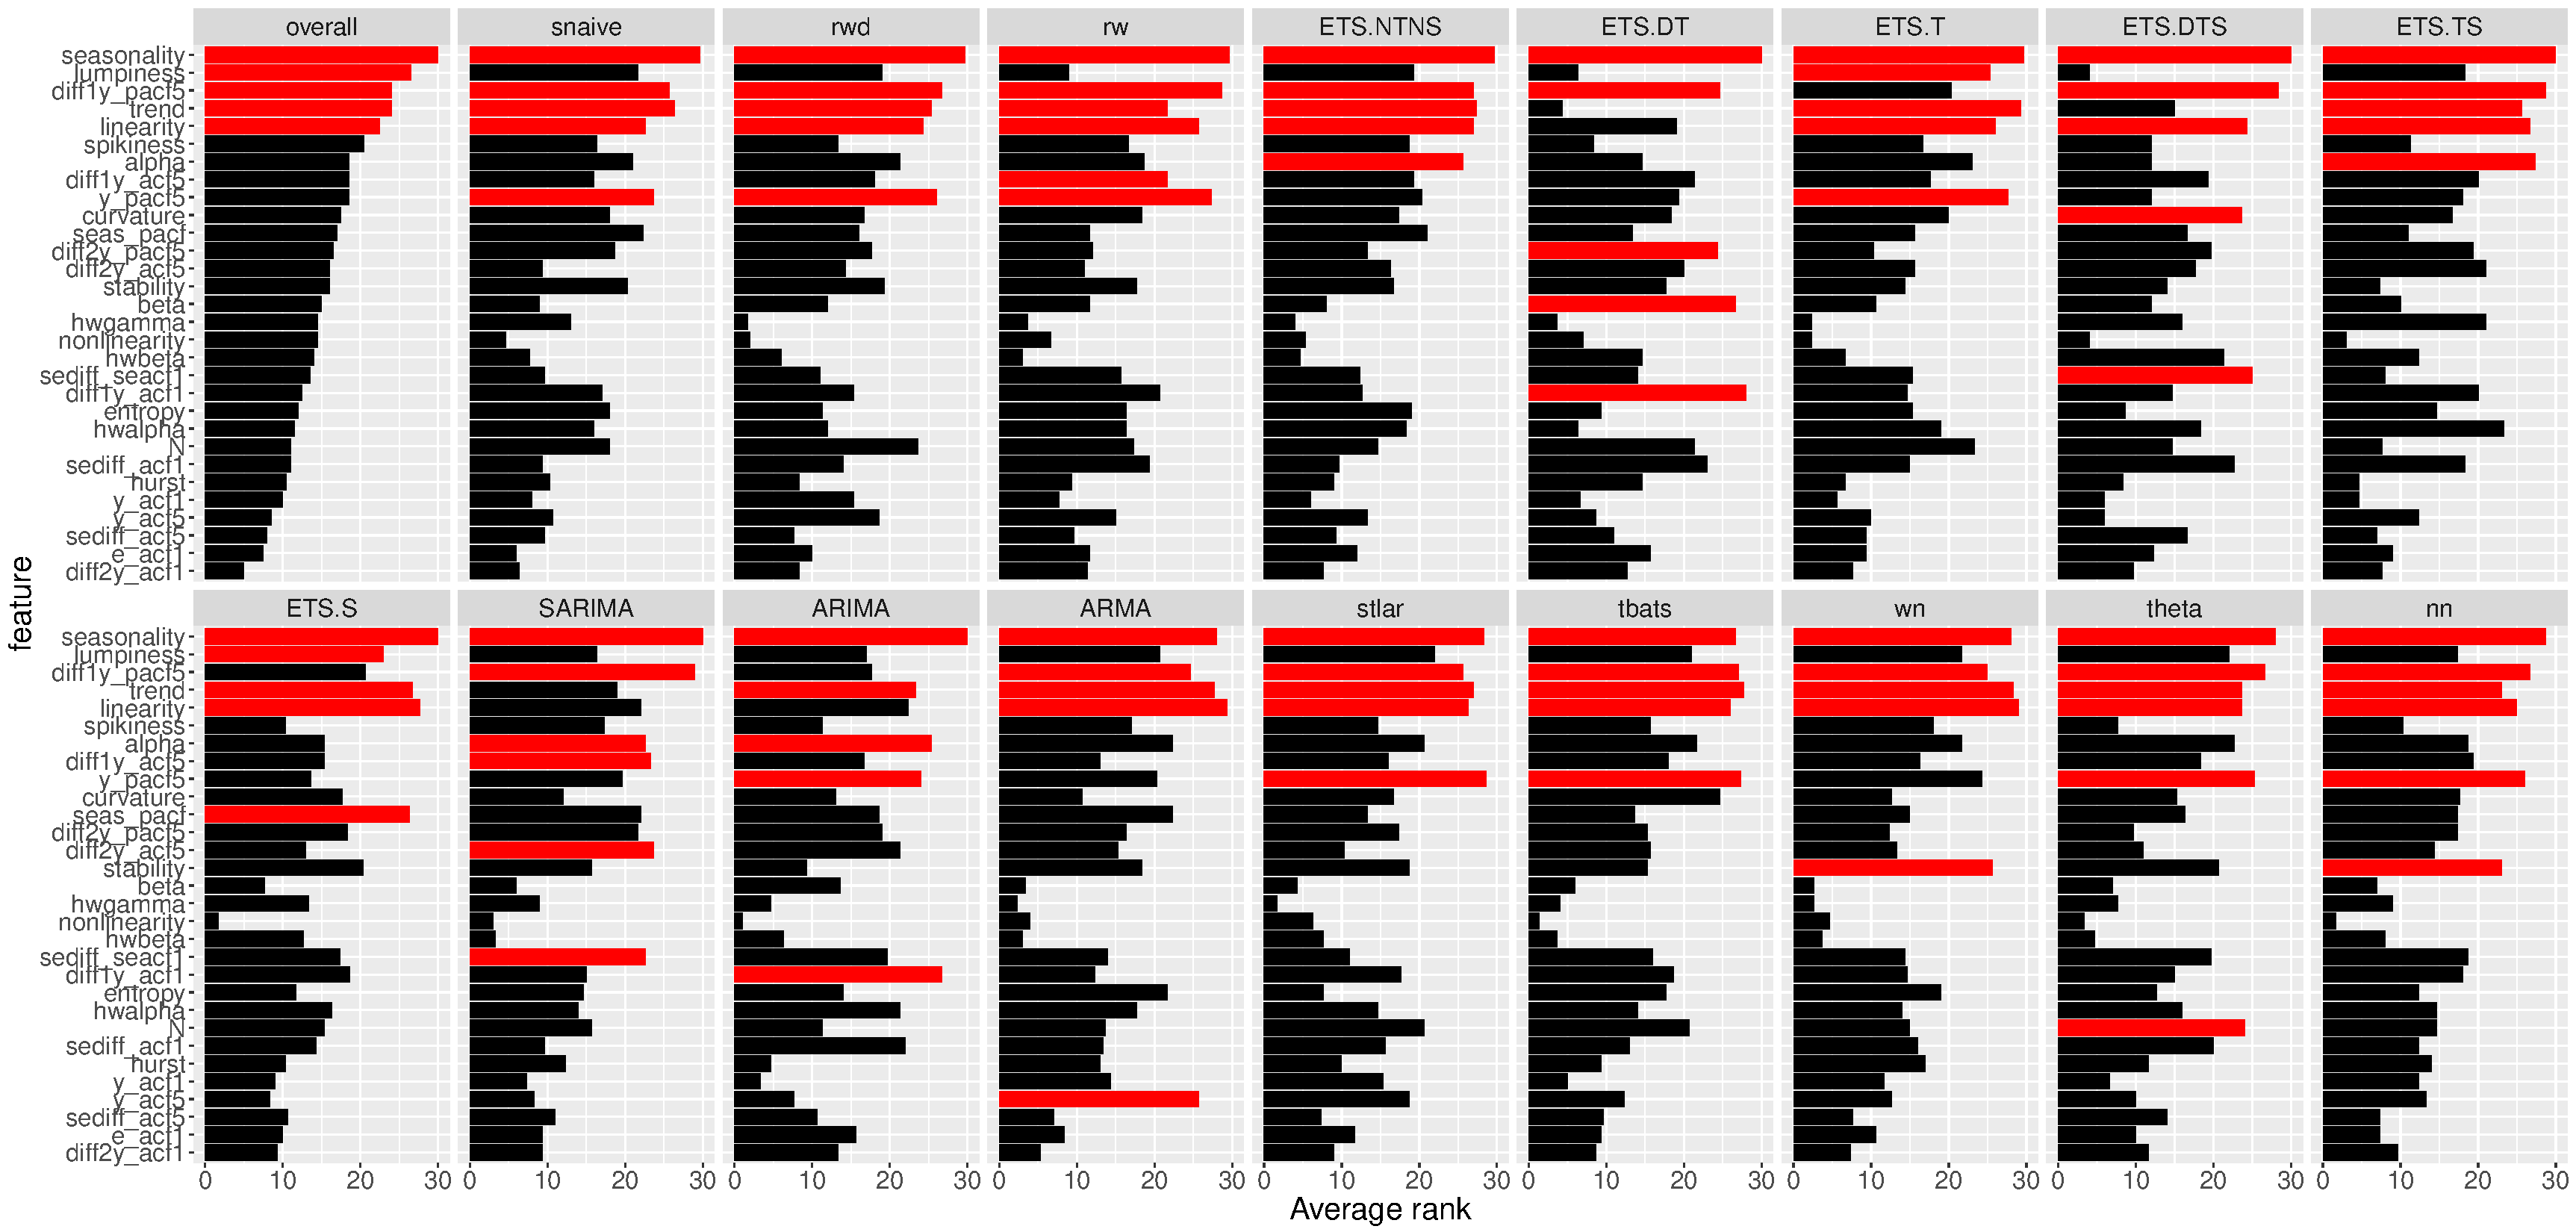
\includegraphics{figures/viquarterly-1.pdf}
\caption{\label{fig:viquarterly}Feature importance plot for quarterly series. Overall feature importance(top left plot) is evaluated based on two measures: i) Permutation-based variable importance measure and ii) mean decrease in Gini coefficients are used to evaluate shown in the top left plot. Class-specific feature importance is evaluated based on three measures: i) permutation-based variable importance, PD-based variable importance measure, and ICE-based variable importance measure. Longer bars indicate more important features. Top 5 overall features are highlighted in purple. Strength of seasonality appears to be the most important feature.}
\end{figure}

\begin{figure}
\centering
\includegraphics{figures/pdpquarterlyseasonality-1.pdf}
\caption{\label{fig:pdpquarterlyseasonality}Partial dependence plots for strength of seasonality (seasonality\_Q). The shading shows the 95\% confidence intervals. Y-axis denotes the probability of belong to corresponding class. Probability of selecting forecast-models with seasonal components increases as seasonality increases.}
\end{figure}

\begin{figure}
\centering
\includegraphics{figures/pdpquarterlydiff1ypacf5-1.pdf}
\caption{\label{fig:pdpquarterlydiff1ypacf5}Partial dependence plots for sum of squares of first 5 PACF values of differenced series (diff1y\_pacf5). The shading shows the 95\% confidence intervals. Y-axis denotes the probability of belong to corresponding class. Probability of selecting SARIMA models drastically increases as diff1y\_pacf5 increases}
\end{figure}

\begin{figure}
\centering
\includegraphics{figures/pdpquarterlytrend-1.pdf}
\caption{\label{fig:pdpquarterlytrend}Partial dependence plots for strength of trend (trend). The shading shows the 95\% confidence intervals. Y-axis denotes the probability of belong to corresponding class. The information about whether a seies has an extremely high trend value or not drastically influence the decision of selecting a forecast-model.}
\end{figure}

According to \autoref{fig:friedmanq} strength of seasonality shows extremely low interactivity within SARIMA, ETS\_DT and ETS\_DTS, indicating the importance of main effect of seasonality within those classes. Only stlar, ETS\_TS and ETS\_S classes show high level of interactivity (\textgreater{} 0.6) for seasonality. ARMA class shows a very low interactivity with y\_acf1, reflecting the importance of y\_acf1 on its own when deciding the probability of selecting ARMA models. Stength of trend show appear to be among top interacting feature within many classes. The interaction strength of trend within random walk and nn are relatively high (\textgreater{} 0.8) compared to others. Length of time series show a high level of interactivity within random walk class.

\begin{figure}
\centering
\includegraphics{figures/intquarterly-1.png}
\caption{\label{fig:intquarterly}Partial dependence plot of model selection probability and the interaction of curvature and e\_acf1 for yearly data. Dark regions show the high probability of belonging to the corresponding class shown in the plot title.}
\end{figure}

\hypertarget{monthly-series}{%
\subsection{Monthly series}\label{monthly-series}}

\autoref{fig:oobmonthly} shows the vote-matrix information for monthly series. Vote matrix information for monthly data depicted similar pattern to quarterly data. For quarterly and monthly data, the same set of features and the class-labels are used to train the model. Hence, this consistency between the results of the quarterly and the monthly series would provide evidence in support of the validity and trustability of the model.

\autoref{fig:vimonthly} shows the feature importance plots for monthly data. For both quarterly and monthly data strength of seasonality, trend, linearity and spikiness are the most important features across all categories. In the case of yearly series low variable importance is assigned to both stability and length of the series. However, within quarterly and monthly data a high variable importance is assigned to length of the series and stability. In addition to the strength of seasonality, the models handling seasonal components (snaive, SARIMA, all ETS models with seasonal component) assigned a high importance to the additional features related to seasonality such as ACF, PACF-based features related to seasonal lag or seasonally differenced series. Furthermore, as expected features calculated based on parameter estimated of ETS(A, A, A) ranked as important for the choice of ETS with damped trend and seasonal component and ETS with trend and seasonal component. One notable difference between the quarterly series and the monthly series is, for monthly data length of the series is ranked among the top five, specially in random walk with drift, random walk, ETS with seasonal and trend component, ETS\_seasonal, SARIMA and ARIMA classes.

\begin{figure}
\centering
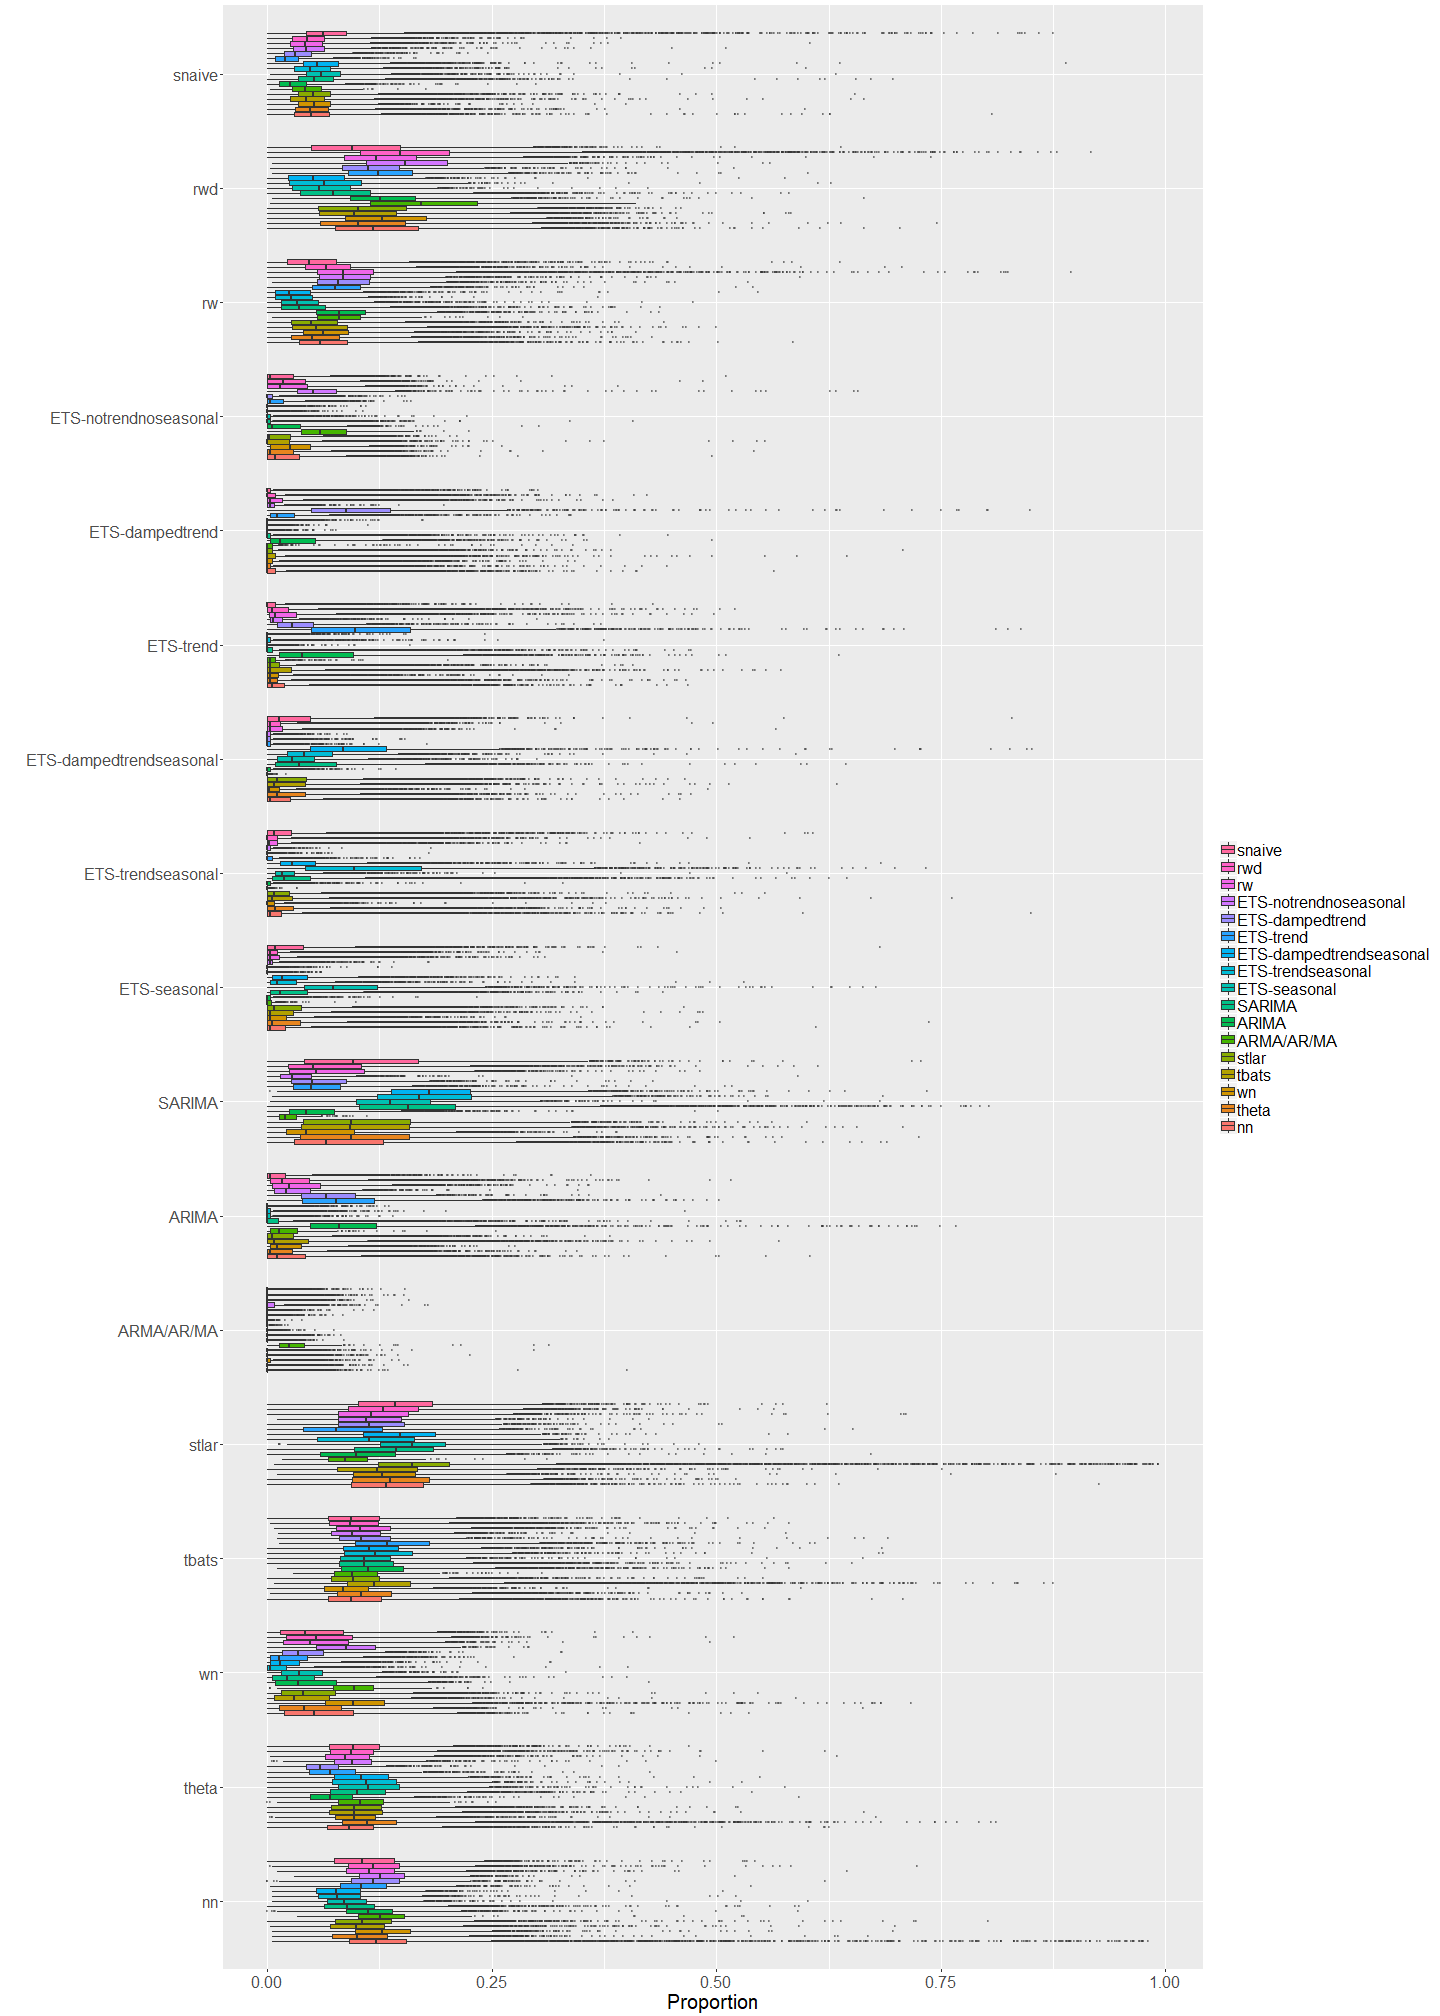
\includegraphics{figures/oobmonthly-1.png}
\caption{\label{fig:oobmonthly}Visualization of the vote matrix based on OOB sample for quarterly random forest. Each panel shows the predicted class from the random forest. The X-axis denotes the proportion of times each time series was classified to each class. The colours of boxplots correspond to class label of the ``best'' forecast-model identified based on MASE and sMAPE. On each row, distribution of correctly classified class dominates, indicating a good classification of the meta-learner.}
\end{figure}

\begin{figure}
\centering
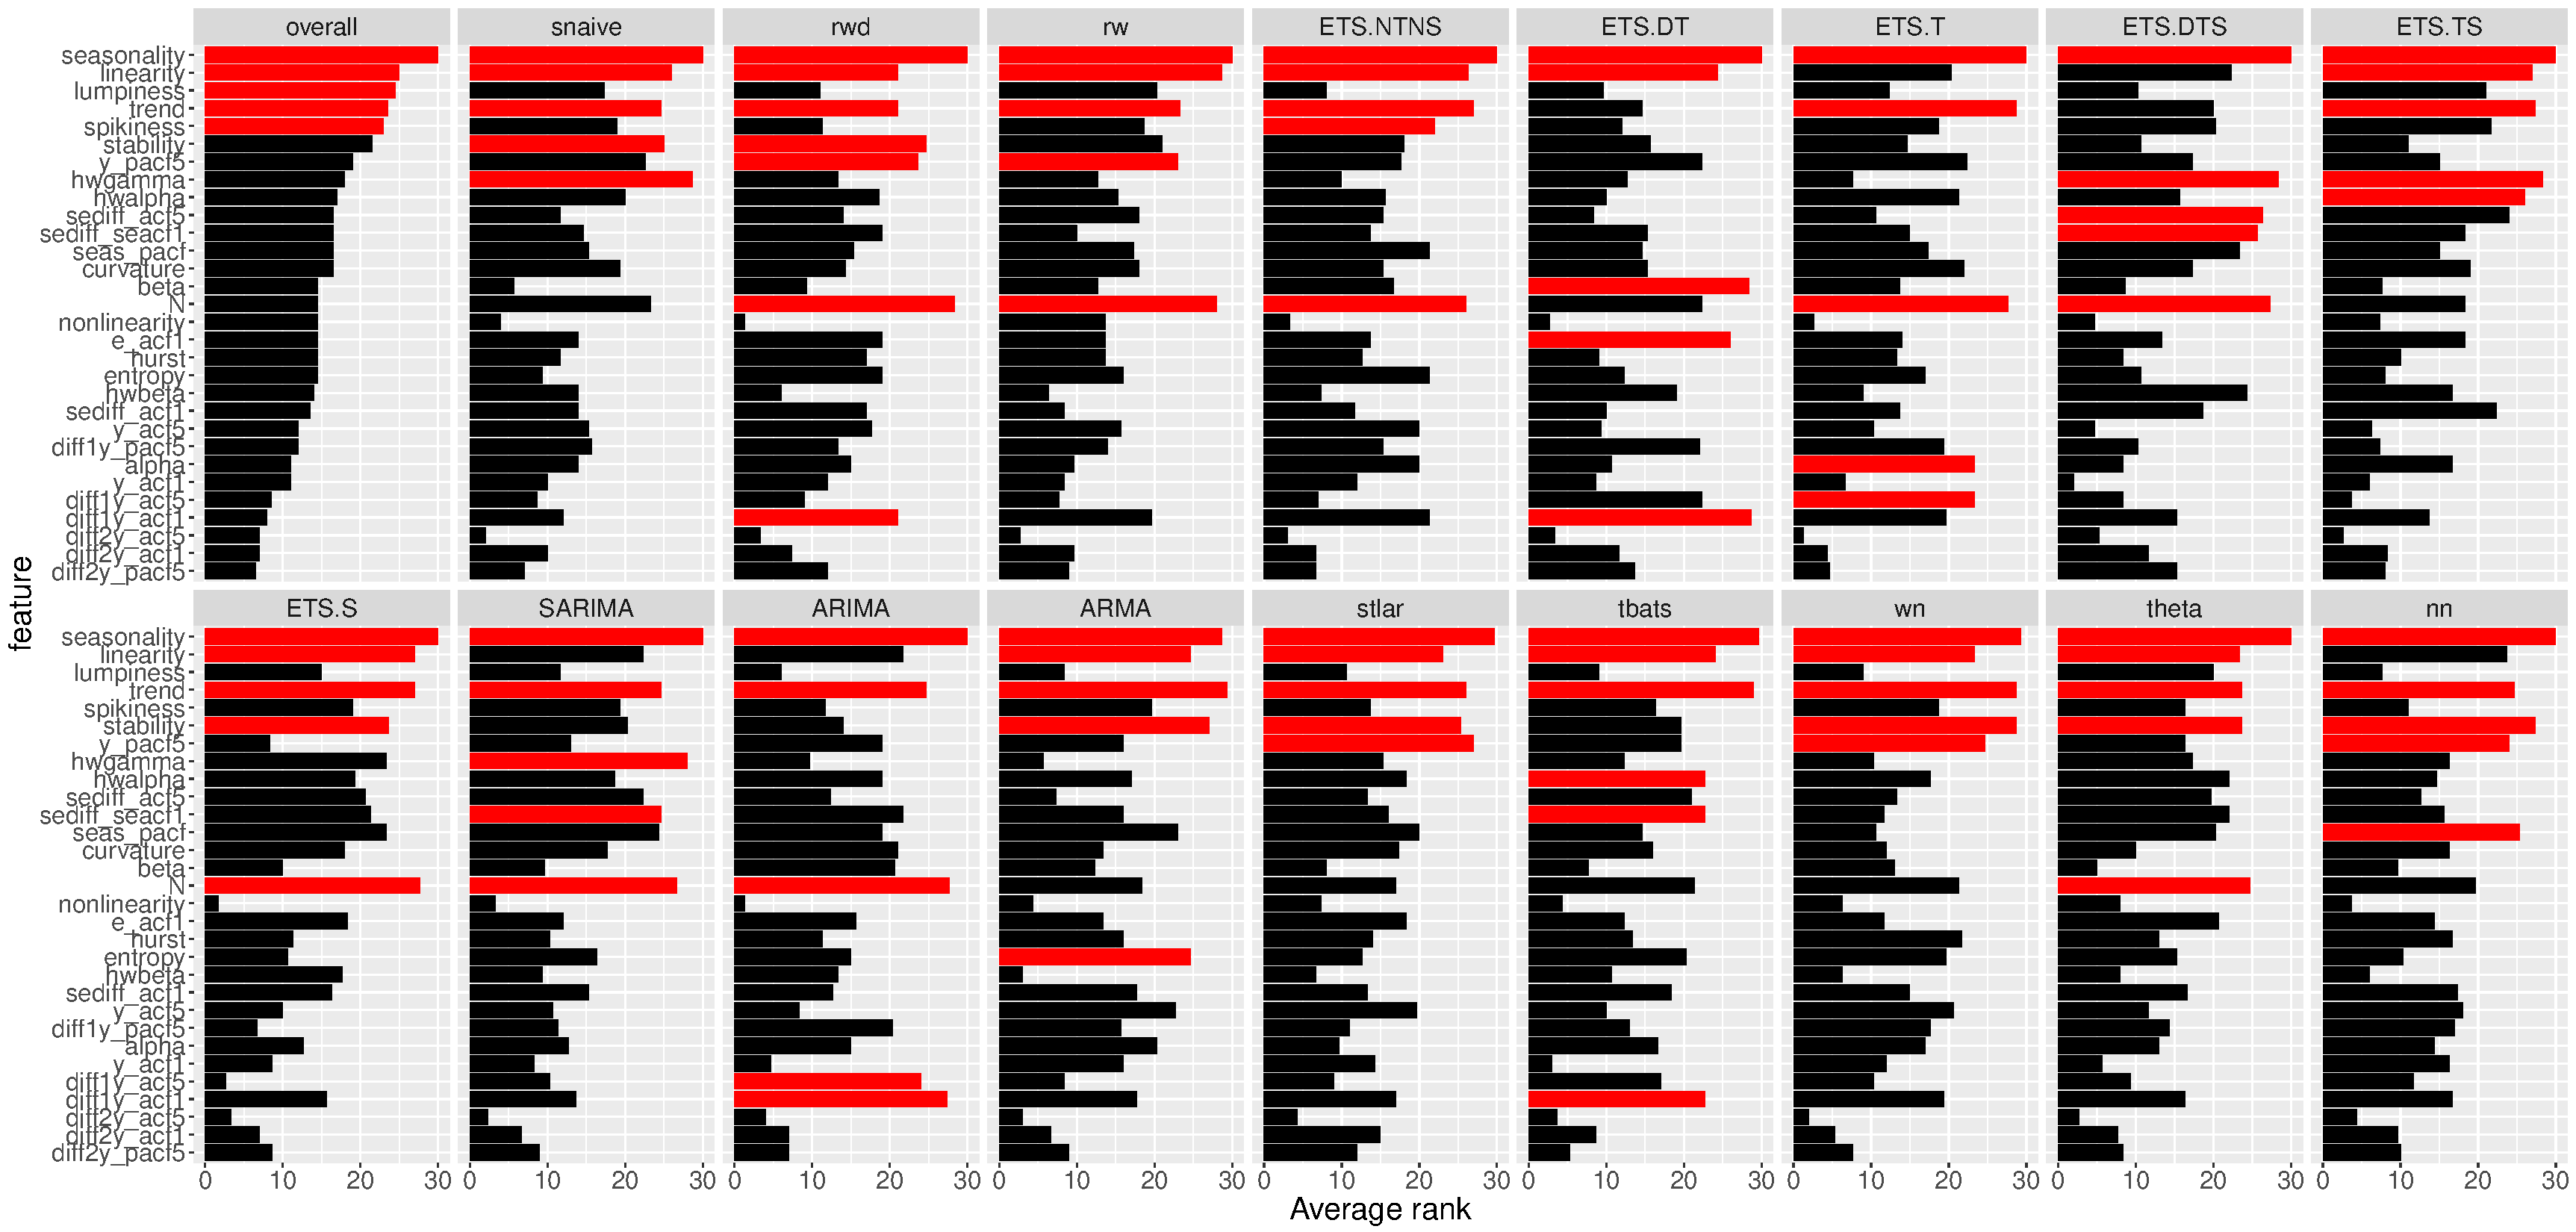
\includegraphics{figures/vimonthly-1.pdf}
\caption{\label{fig:vimonthly}Feature importance plot for monthly series. Overall feature importance(top left plot) is evaluated based on two measures: i) Permutation-based variable importance measure and ii) mean decrease in Gini coefficients are used to evaluate shown in the top left plot. Class-specific feature importance is evaluated based on three measures: i) permutation-based variable importance, PD-based variable importance measure, and ICE-based variable importance measure. Longer bars indicate more important features. Top 5 overall features are highlighted in purple. Strength of seasonality appears to be the most important feature.}
\end{figure}

\begin{figure}
\centering
\includegraphics{figures/pdpmonthlylinearity-1.pdf}
\caption{\label{fig:pdpmonthlylinearity}Partial dependence plots for linearity. The shading shows the 95\% confidence intervals. Y-axis denotes the probability of belong to corresponding class. All curves show an turning point in the relationship around zeo.}
\end{figure}

\begin{figure}
\centering
\includegraphics{figures/pdpmonthlyN-1.pdf}
\caption{\label{fig:pdpmonthlyN}Partial dependence plots for length of time series (T). The shading shows the 95\% confidence intervals. Y-axis denotes the probability of belong to corresponding class. Probability of selecting rw and rwd decreases as the length \textgreater{} 500.}
\end{figure}

The partial dependency curves of seasonality and trend of monthly data are very similar to the corresponding plots of quarterly data. Hence, these partial dependency curves are not repeated here. \autoref{fig:pdpmonthlylinearity} partial dependency plot of linearity for monthly data. For non-seasonal forecast models the relationships are very similar to the corresponding observed curves in yearly data. Partial dependency curves of \autoref{fig:pdpmonthlyN} reveals highly parameterized models and models involves seasonal components such as (ETS\_TS, ETS\_DTS, ETS\_S, SARIMA, tbats) shows an increasing relationship with N after some point. According to figure \autoref{fig:friedmanm} we can see number of features show high level(\textgreater{}0.5) of interactivity within classes are relatively low.

\begin{figure}
\centering
\includegraphics{figures/intmonthly-1.png}
\caption{\label{fig:intmonthly}Partial dependence plot of model selection probability and the interaction of linearity and curvature for yearly data. Dark regions show the high probability of belonging to the corresponding class shown in the plot title.}
\end{figure}

\hypertarget{weekly-series}{%
\subsection{Weekly series}\label{weekly-series}}

\autoref{fig:oobweekly} shows the vote matrix information for weekly data. Unlike, yearly, quarterly and monthly data theta method has a low chance of getting selected. The random walk with drift, tbats models and nn have a high chance of getting selected. ARMA class shows some unusual behaviour within some categories due to class imbalance ratio, ARMA class contains fewer number of observations in the training set.

\begin{figure}
\centering
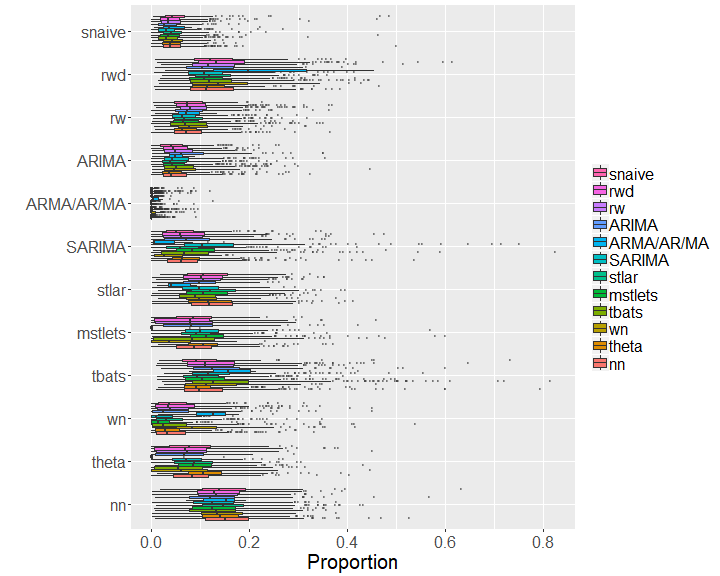
\includegraphics{figures/oobweekly-1.png}
\caption{\label{fig:oobweekly}Visualization of the vote matrix based on OOB sample for weekly random forest. The Y-axis denotes what was predicted from the random forest. The X-axis denotes the proportion of times each time series was classified to each class. The colours of boxplots corresponds to class label of the ``best'' forecast-model identified based on MASE and sMAPE. The models rwd, tbats, nn have a high chance of getting selected.}
\end{figure}

According to the results of \autoref{fig:viweekly} spikiness, linearity, trend, strength of seasonality, stability and lumpiness have been assigned a high importance. This is similar to the results of yearly, quarterly and monthly data. The length of series has been selected among top 5 by mstlets, tbats, theta and neural network models. The partial dependence plots for seasonality, trend and linearity is very similar to the patterns observed in quarterly and monthly data. Hence, we have not repeated the results. Instead, we have plotted the partial dependence plot for spikiness. According to \autoref{fig:weeklypdp} the probability of selecting snaive, random walk, neural network and white noise increases as the spikiness increases while other forecast-model classes show the opposite.

\begin{figure}[h]

{\centering 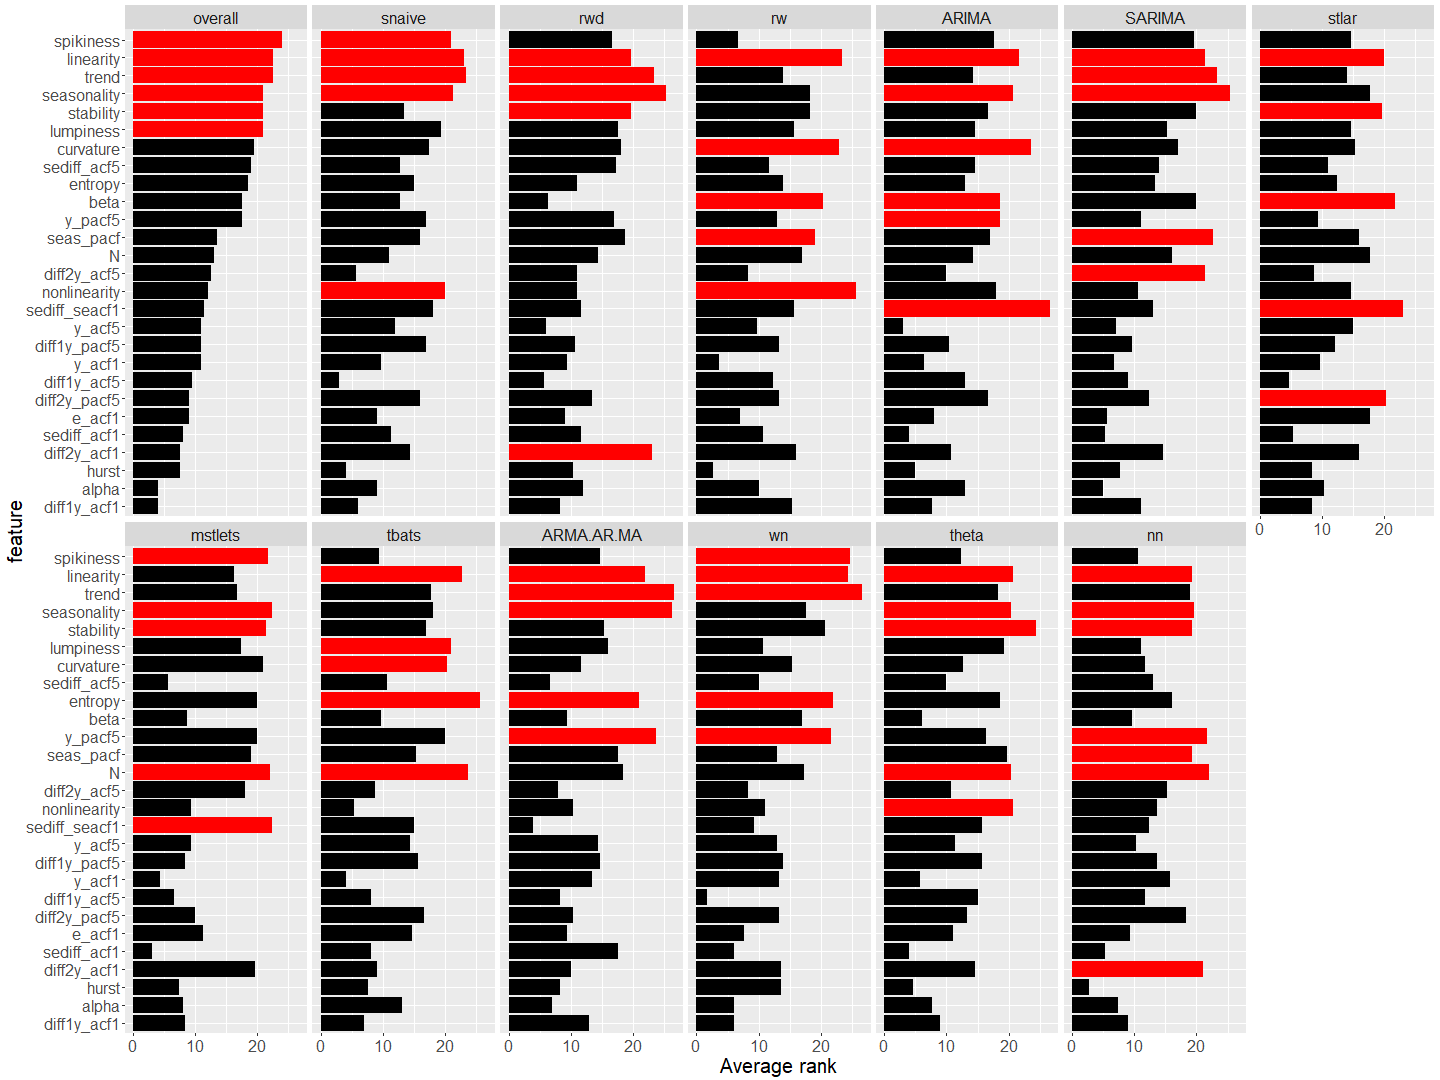
\includegraphics{figures/viweekly-1} 

}

\caption{Feature importance plot for weekly data. Permutation-based VI measure and mean decrease in Gini coefficient is used to evaluate overall feature importance. Class-specific feature importance is evaluated based on the three measures: permutation-based VI, PD-based VI measure, and ICE-based VI measure. Longer bars indicate more important features. Top 5 features are highlighted in purple.}\label{fig:viweekly}
\end{figure}

\begin{figure}
\centering
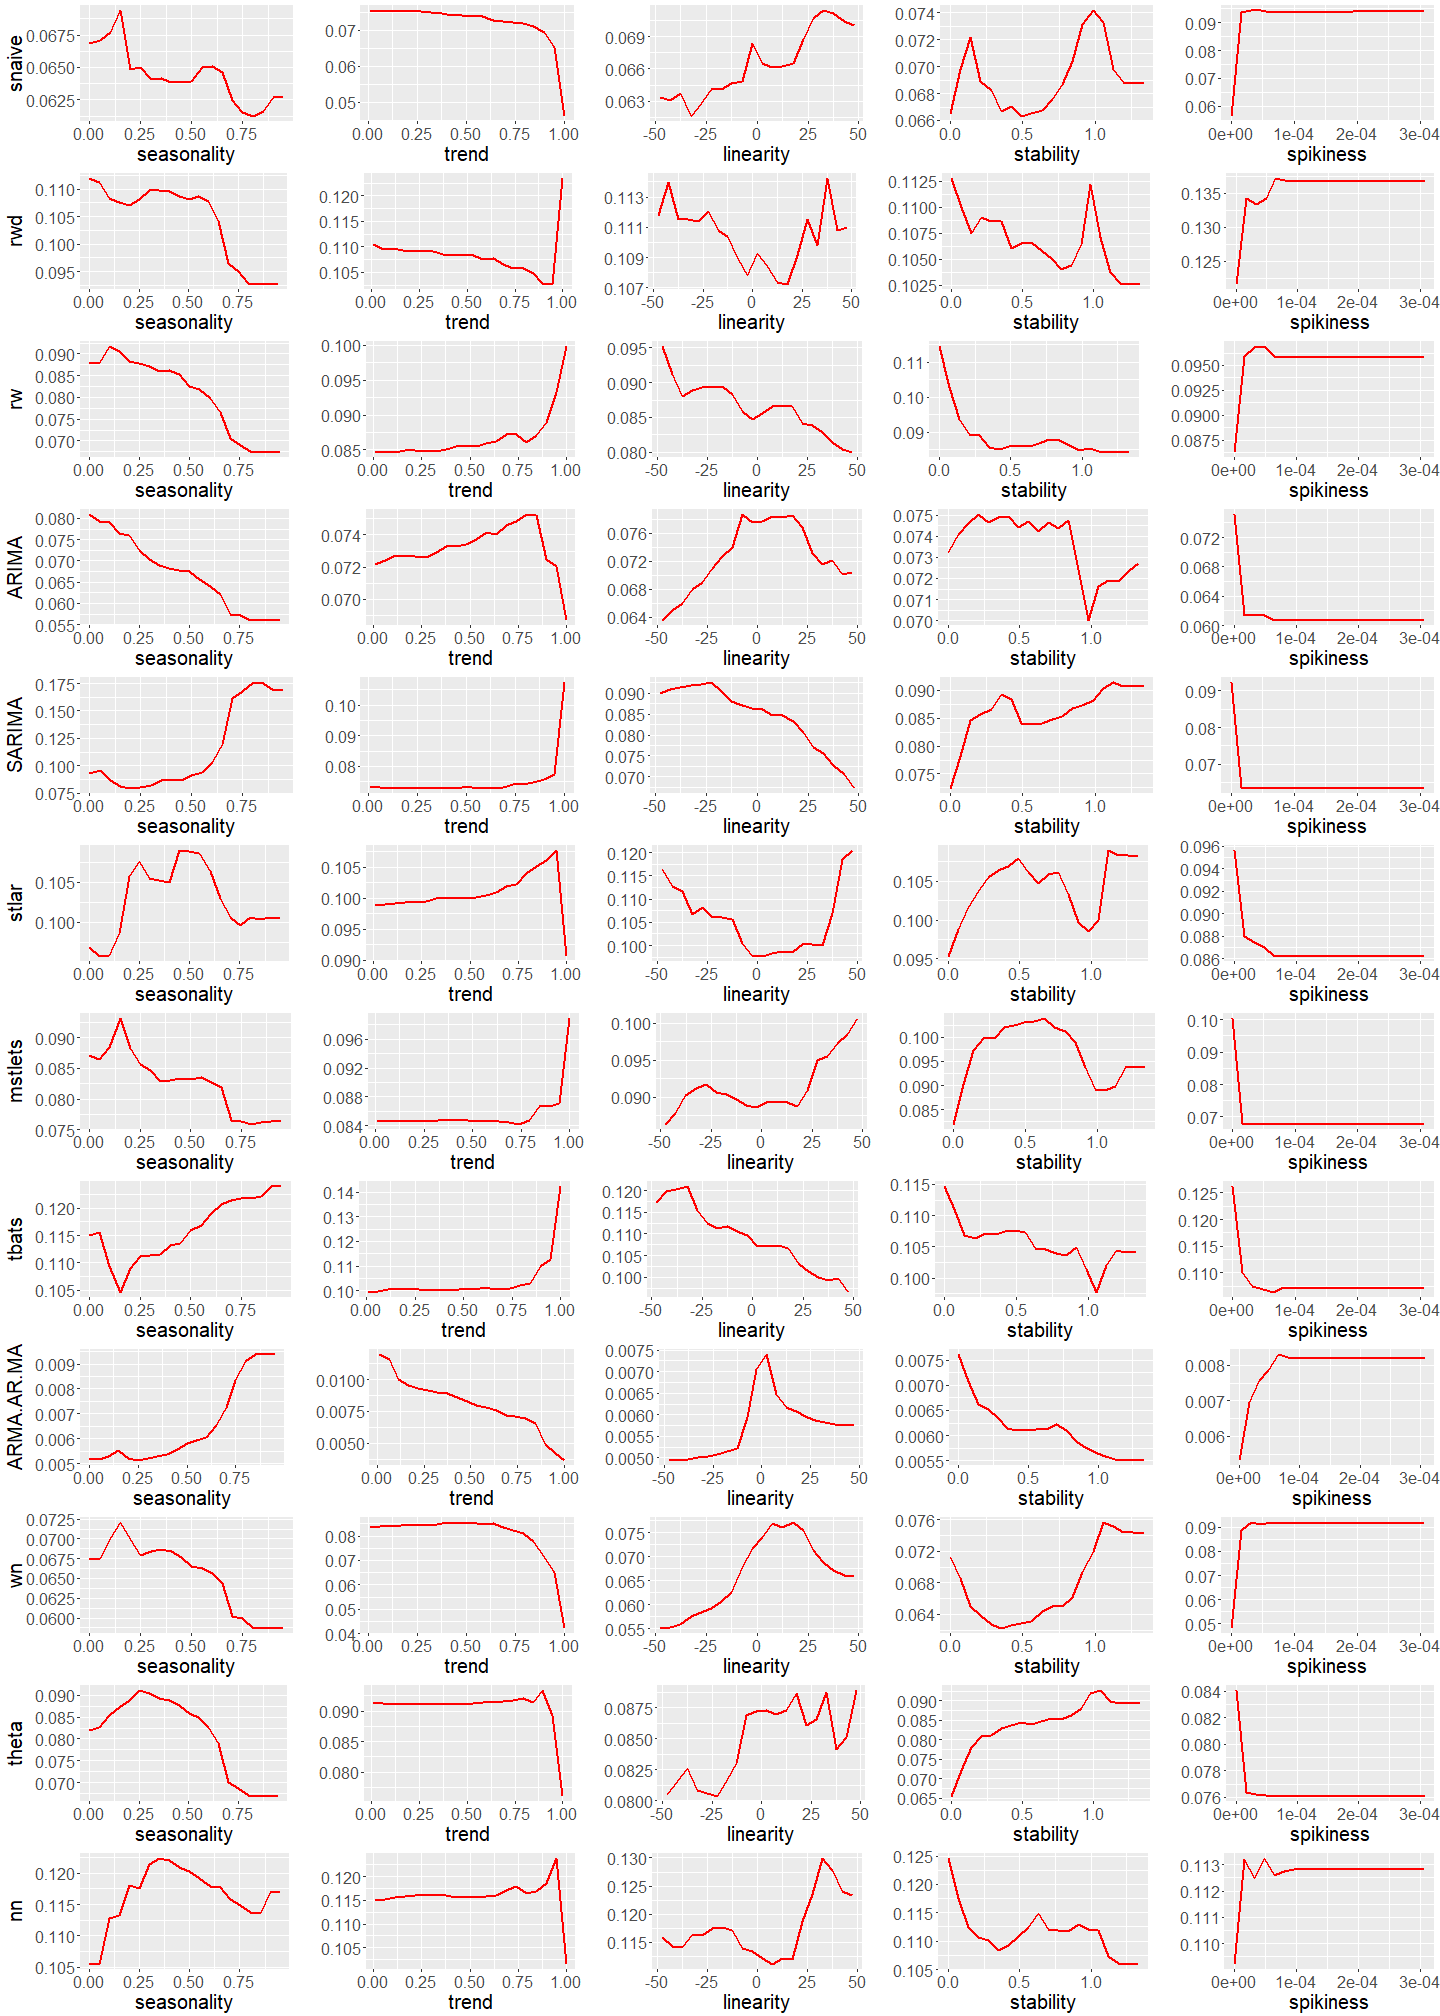
\includegraphics{figures/weeklypdp-1.pdf}
\caption{\label{fig:weeklypdp}Partial dependence plots for the top ranked features from variable importance measures (weekly series). The shading shows the 95\% confidence intervals. Y-axis denotes the probability of belonging to corresponding class.}
\end{figure}

Overall strength of interaction effect for features are shown in \autoref{fig:friedmanw}. Except, ARMA class for all other features across different classes strength of interaction is relatively low (\textless{} 0.25). This reflects the importance of individual effect of features when selecting forecast-models for weekly data.

\begin{figure}
\centering
\includegraphics{figures/intweekly-1.png}
\caption{\label{fig:intweekly}Partial dependence plot of model selection probability and the interaction of curvature and linearity for yearly data. Dark regions show the high probability of belonging to the corresponding class shown in the plot title.}
\end{figure}

\hypertarget{daily-series}{%
\subsection{Daily series}\label{daily-series}}

\autoref{fig:oobdaily} shows the vote matrix information for hourly data. According to \autoref{fig:oobdaily} the distributions corresponds to observations that have been correctly classified dominate the top for daily data. However, within daily series there are few observations that have been incorrectly classified to tbats class with very high probabilities. In general, neural network models have a higher chance of getting selected for daily time series.

Variable importance graph for daily data is shown in \autoref{fig:vidaily}. The most important features for daily time series are, strength of seasonality corresponds to the weekly seasonality (7, measured by seasonal\_strength1), stability, trend, lumpiness and linearity. Furthermore, length of the series is important in determining random walk, random walk with drift, mstlarima, mstlets, stlar, theta and nn classes.

\autoref{fig:dailypdpstability} we can see probability of selecting white noise models increases as stability increases. According to the partial dependency curves of length(N)
\autoref{fig:dailypdpstability} shorter series tends to select random walk with drift models while probability of selecting snaive, mstlarima and mstlets models increases as the length of series increases. Neural network models show a non-monotonic relationship with length of the series (N). The theta models tend to be selected for series with high annual seasonality but
very low weekly seasonality.

\begin{figure}
\centering
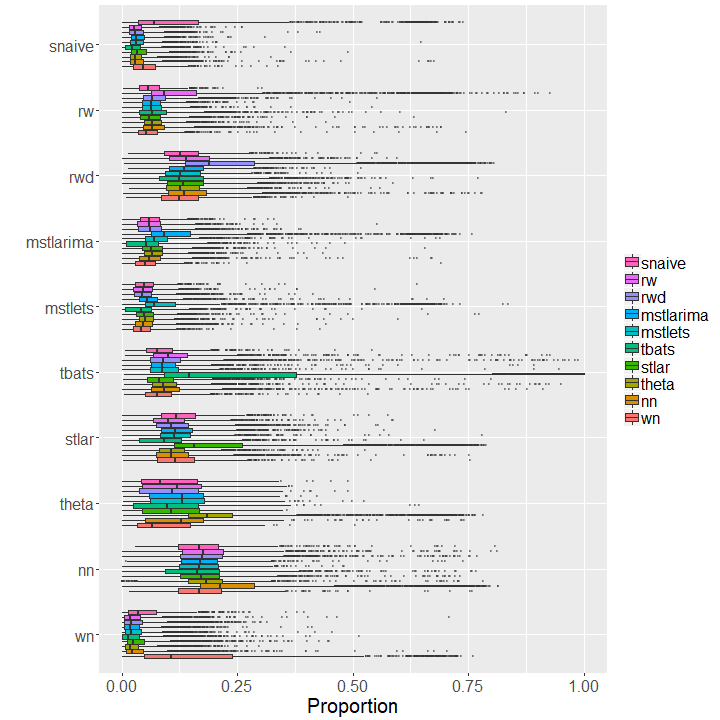
\includegraphics{figures/oobdaily-1.png}
\caption{\label{fig:oobdaily}Visualization of the vote matrix based on OOB sample for daily random forest. The Y-axis denotes what was predicted from the random forest. The X-axis denotes the proportion of times each time series was classified to each class. The colours of boxplots corresponds to class label of the ``best'' forecast-model identified based on MASE and sMAPE. The models rwd, tbats, nn have a high chance of getting selected.}
\end{figure}

\begin{figure}[h]

{\centering 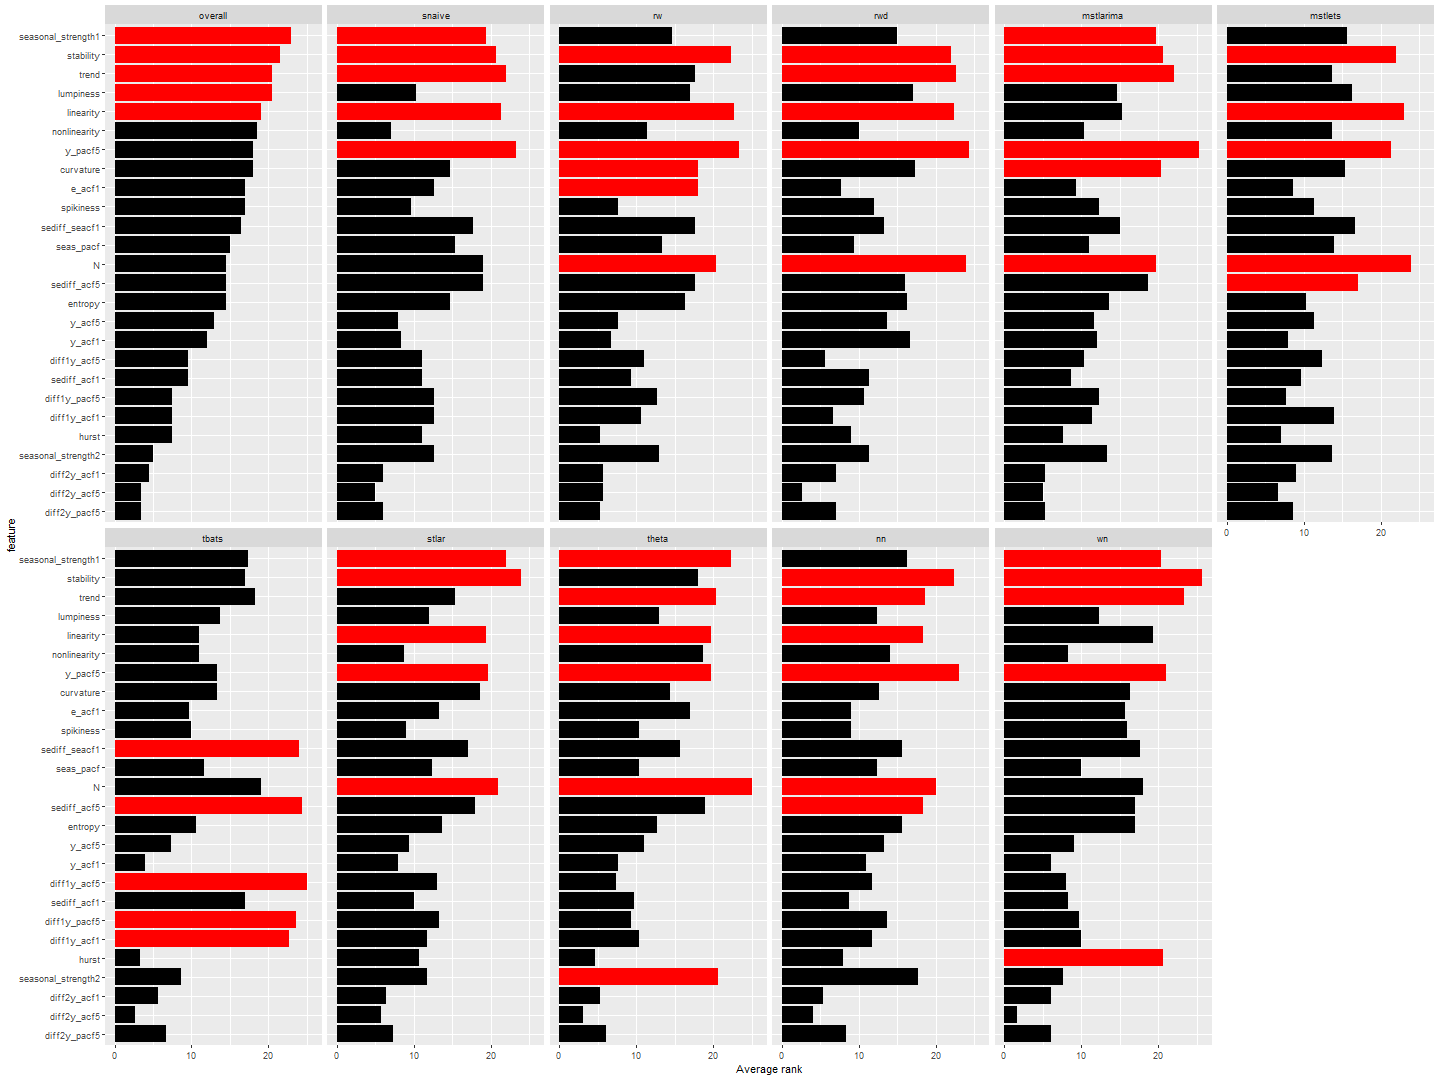
\includegraphics{figures/vidaily-1} 

}

\caption{Feature importance plot for daily data. Permutation-based VI measure and mean decrease in Gini coefficients are used to evaluate overall feature importance. Class-specific feature importance is evaluated based on the three measures: permutation-based VI, PD-based VI measure, and ICE-based VI measure. Longer bars indicate more important features. Top 5 features are highlighted in red.}\label{fig:vidaily}
\end{figure}

According to \autoref{fig:friedmand} number of features that show high level of interactivity (\textgreater{}0.7) with other features are relatively low. Friedman's H-statistic for most of the features across different categories are roughly around o.25, meaning that 25\% of variation is explained by the interaction effect.

\begin{figure}
\centering
\includegraphics{figures/dailypdpstability-1.pdf}
\caption{\label{fig:dailypdpstability}Partial dependence plots for stability. The shading shows the 95\% confidence intervals. Y-axis denotes the probability of belonging to corresponding class.}
\end{figure}

\begin{figure}
\centering
\includegraphics{figures/dailypdpN-1.pdf}
\caption{\label{fig:dailypdpN}Partial dependence plots for stability. The shading shows the 95\% confidence intervals. Y-axis denotes the probability of belonging to corresponding class.}
\end{figure}

\begin{figure}
\centering
\includegraphics{figures/intdaily-1.png}
\caption{\label{fig:intdaily}Partial dependence plot of model selection probability and the interaction of sediff\_seacf1 and linearity for hourly data. Dark regions show the high probability of belonging to the corresponding class shown in the plot title. Random walk and random walk with drift class show opposite pattern of interactivity between sediff\_seacf1 and linearity.}
\end{figure}

\hypertarget{hourly-series}{%
\subsection{Hourly series}\label{hourly-series}}

\autoref{fig:oobhourly} shows the vote matrix information for hourly data. Overall, for hourly series random walk with drift models, tbats and neural network models have a high chance of getting selected. Furthermore, it is important to note that within nn panels all distributions located away from series which indicates all hourly series have been assigned a non-zero probability of getting selected to neural network class.

Variable importance graph for hourly data is shown in \autoref{fig:vihourly}. According to \autoref{fig:vihourly}, the strength of daily seasonality (period=24, measured by seasonal\_strength1) appear to be more important than the strength of weekly seasonality (period=168, measured by seasonal\_strength2). However, the strength of weekly seasonality also seems to be one of the most important features for classes snaive, random walk, mstlarima, and tbats. Furthermore, entropy, linearity, sum of squares of first 5 coefficients of PACF, curvature, trend, spikiness and stability were found to be the most important features in determining best forecasting method for hourly time series. Only snaive category ranked N among top 5 for hourly time series.

The partial dependency plots of the strength of seasonalities are shown in \autoref{fig:seasonalityhourly}. According to \autoref{fig:seasonalityhourly} the probability of selecting random walk, random walk with drift, theta model and white noise process decrease with higher value of strength of daily seasonality. On the other hand, probability of selecting random walk model increase as the strength of weekly seasonality increases. The partial dependency plots of entropy are shown in \autoref{fig:entropyhourly}. The entropy measures forecastability of time series. We can see the probability of selecting random walk with drift and tbats decreases as the entropy increases. The is consistent with our theoretical expectations. In other words, if the series has a clear trend or a clear trigonometric pattern then the forecastability of the time series is high and the entropy is low. For a clear trend, random walk with drift model is suitable while for a series with trigonometric pattern tbats model is suitable.

According to \autoref{fig:friedmanh} linearity shows high level of interactivity within many classes. Furthermore, we dive deeper into all 2-way interactions with linearity by observing the Friedman's H-Statistics. Friedman's H-Statistic shows high level of interactivity (value close to 1.00) between sediff\_seacf1 and linearity across all classes. The associated two-way partial dependency plot is shown below.

\begin{figure}
\centering
\includegraphics{figures/oobhourly-1.png}
\caption{\label{fig:oobhourly}Visualization of the vote matrix based on OOB sample for hourly random forest. The Y-axis denotes what was predicted from the random forest. The X-axis denotes the proportion of times each time series was classified to each class. The colours of boxplots corresponds to class label of the ``best'' forecast-model identified based on MASE and sMAPE. The models rwd, tbats, nn have a high chance of getting selected.}
\end{figure}

\begin{figure}
\centering
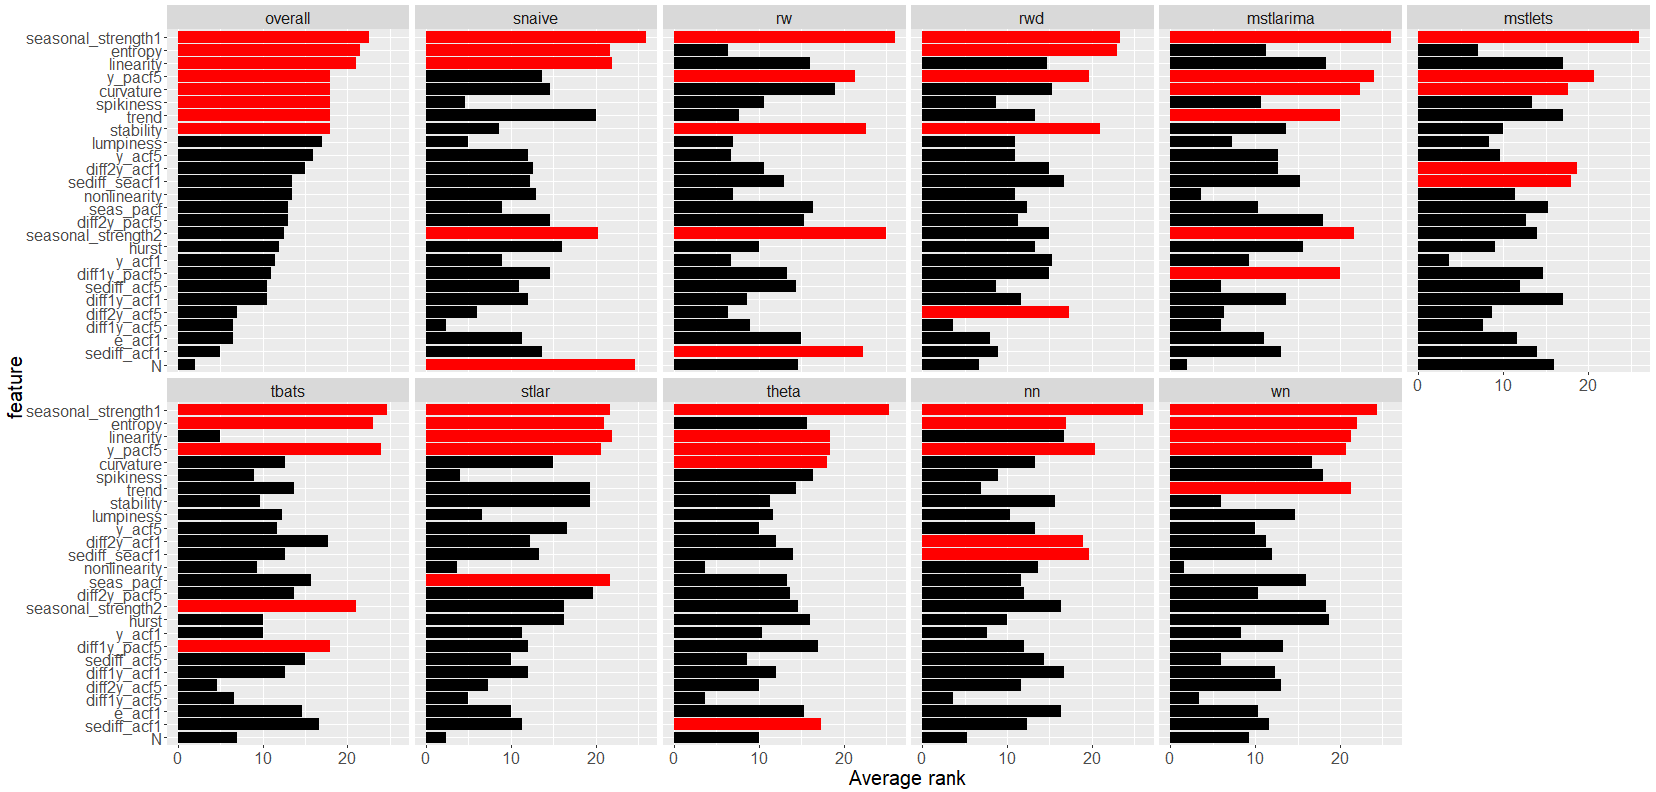
\includegraphics{figures/vihourly-1.pdf}
\caption{\label{fig:vihourly}Feature importance plot hourly series. Permutation-based VI measure and mean decrease in Gini coefficients are used to evaluate overall feature importance. Class-specific feature importance is evaluated based on the three measures: permutation-based VI, PD-based VI measure, and ICE-based VI measure. Longer bars indicate more important features. Top 5 features are highlighted in red.}
\end{figure}

\begin{figure}
\centering
\includegraphics{figures/seasonalityhourly-1.pdf}
\caption{\label{fig:seasonalityhourly}Partial dependence plots for strength of seasonality. The shading shows the 95\% confidence intervals. Y-axis denotes the probability of belonging to corresponding class.}
\end{figure}

\begin{figure}
\centering
\includegraphics{figures/entropyhourly-1.pdf}
\caption{\label{fig:entropyhourly}Partial dependence plots for entropy. The shading shows the 95\% confidence intervals. Y-axis denotes the probability of belonging to corresponding class.}
\end{figure}

\begin{figure}
\centering
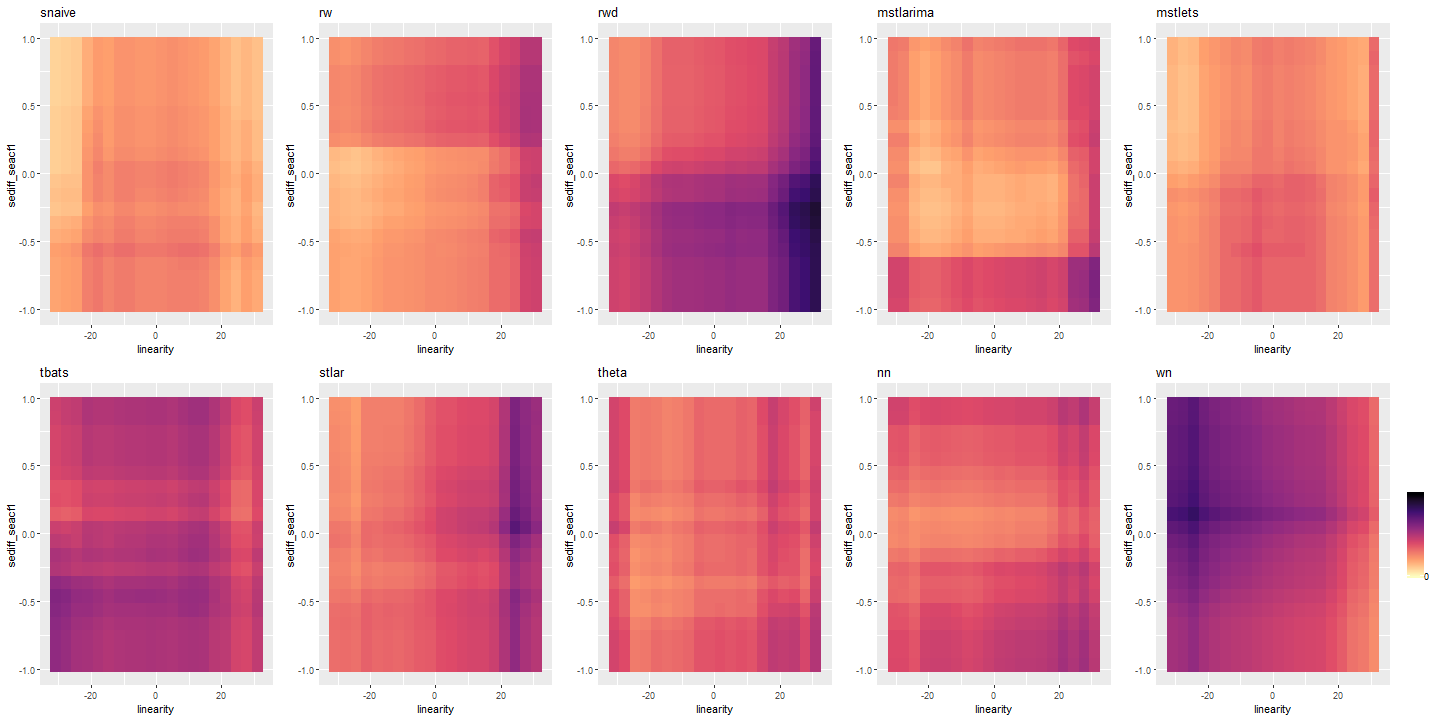
\includegraphics{figures/htwopdp-1.png}
\caption{\label{fig:htwopdp}Partial dependence plot of model selection probability and the interaction of sediff\_seacf1 and linearity for hourly data. Dark regions show the high probability of belonging to the corresponding class shown in the plot title. Random walk and random walk with drift class show opposite pattern of interactivity between sediff\_seacf1 and linearity.}
\end{figure}

\clearpage

\hypertarget{local-interpretable-model-agnostic-explanations}{%
\subsection{Local Interpretable Model-agnostic Explanations}\label{local-interpretable-model-agnostic-explanations}}

\begin{figure}[h]

{\centering 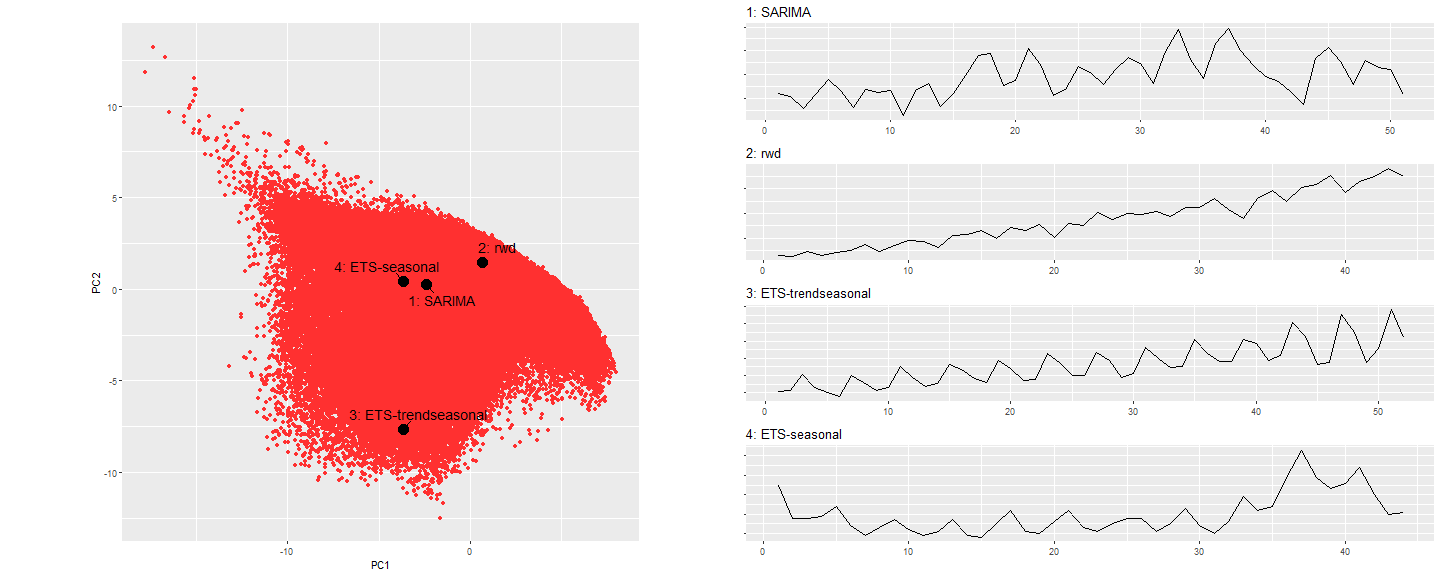
\includegraphics{figures/quarterlylime-1} 

}

\end{figure}

\begin{figure}[h]

{\centering 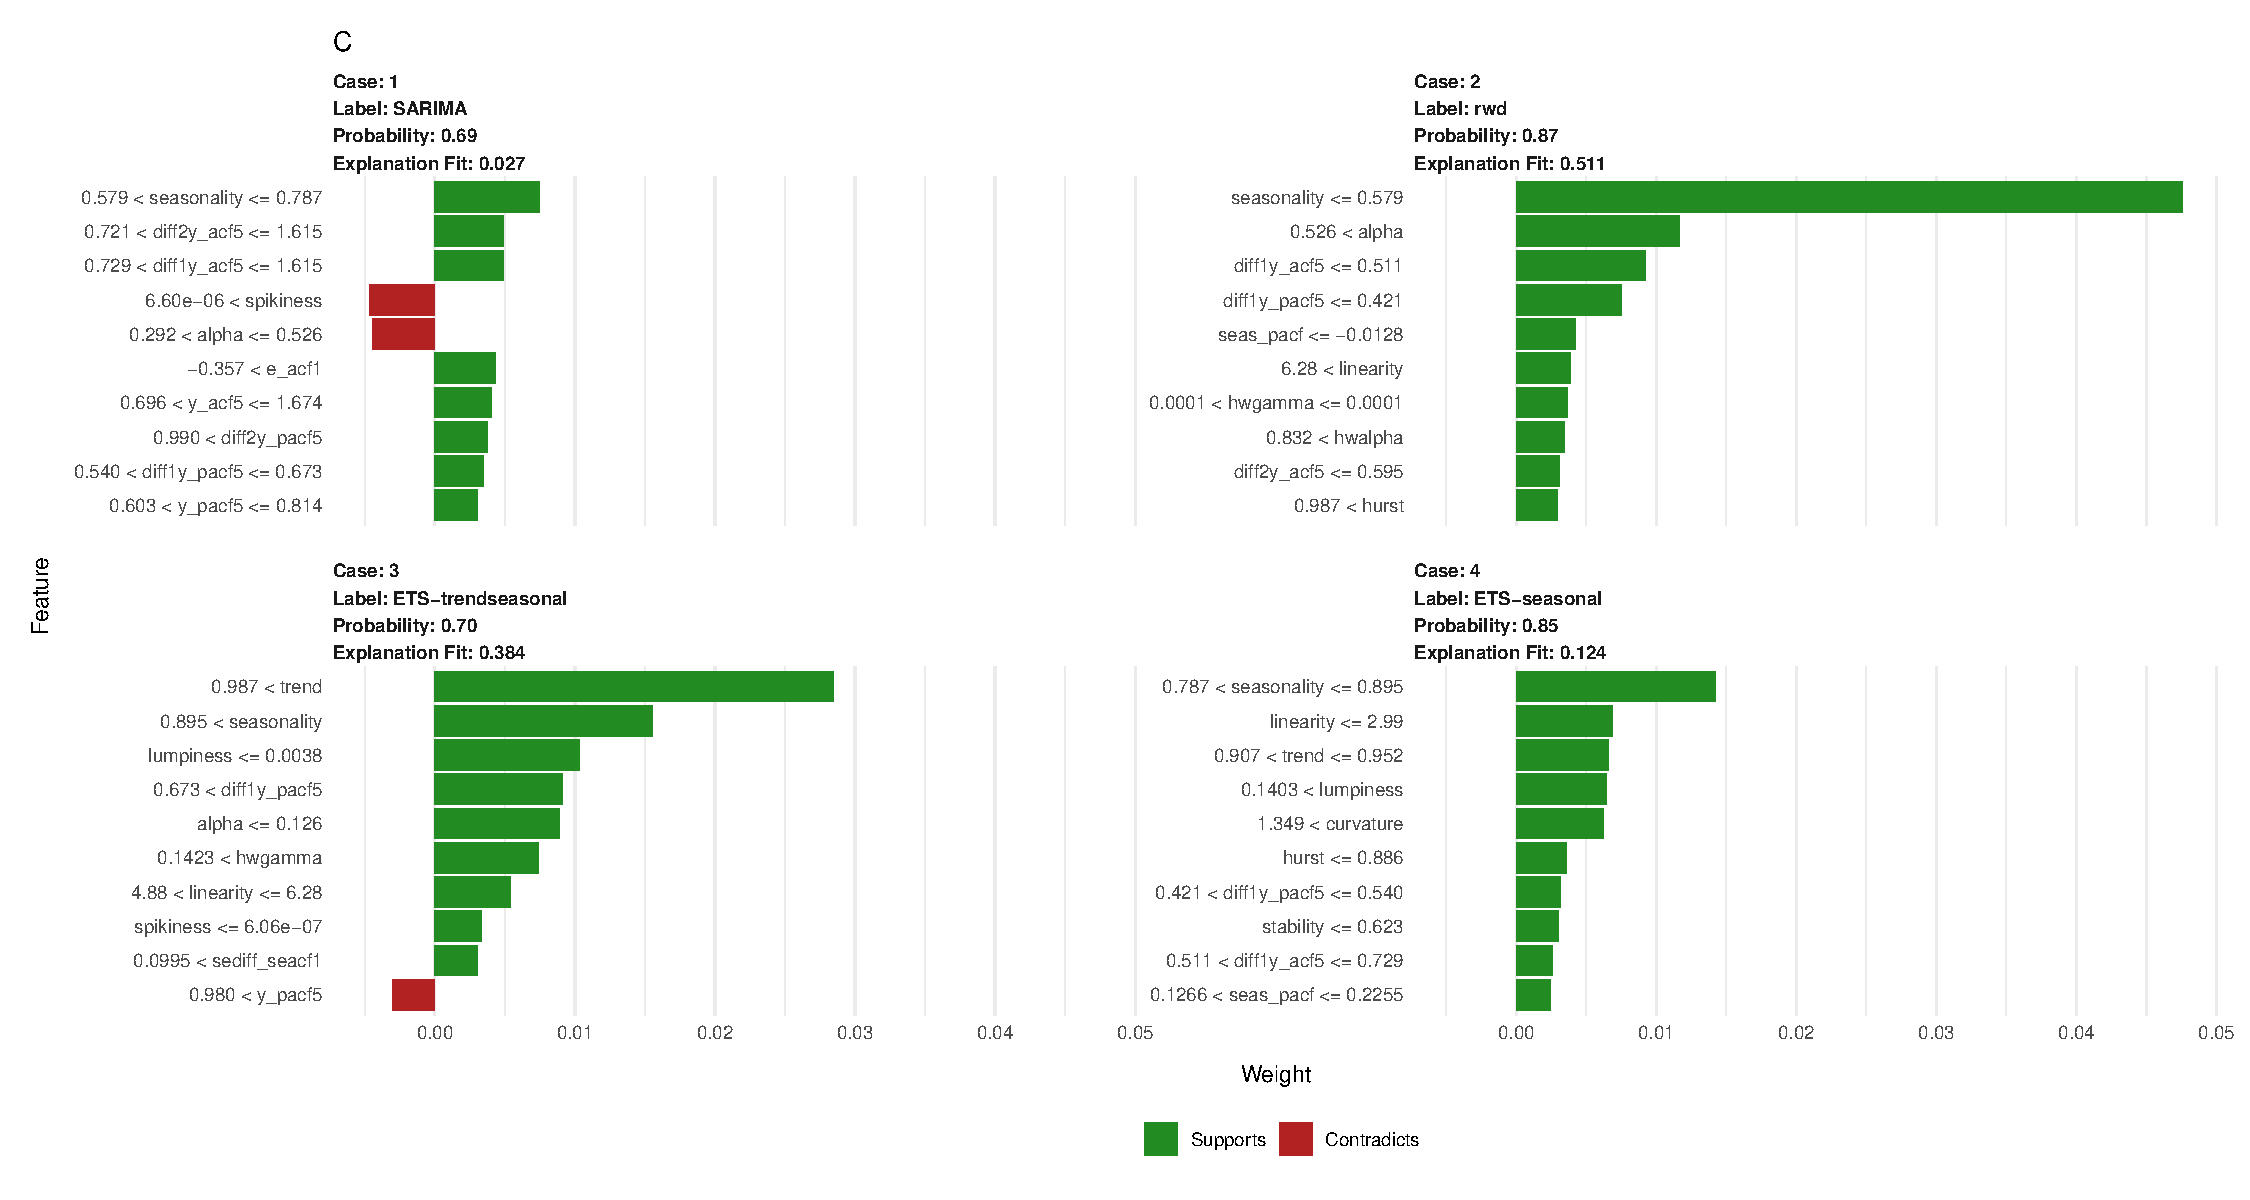
\includegraphics{figures/quarterlylime2-1} 

}

\caption{Panel A: Distribution of quarterly time series in the PCA space. Panel B: Time series corresponds to the highlighted points in the PCA space. Panel C: Local interpretable Model-agnostic explanations for four selected quarterly time series. Features denoted with green colour are supporting features for an outcome label and length of the bar is proportional to the weight of a feature.}\label{fig:quarterlylime2}
\end{figure}

We now illustrate how LIME approach can be used to zoom into local regions of the data to identify which features, contribute most to classify a specific instance. For the illustration we select four different time series classified with high probability. \autoref{fig:quarterlylime2} shows the feature contribution for the instances highlighted on the PCA-space of quarterly series. We can see how the strength of seasonality influences the FFORMS framework to select different types of seasonal forecast-models. For example, SARIMA model is selected when the seasonality varies between 0.579 and 0.787 (case 1), ETS-seasonal model is selected when the strength of seasonality is greater than 0.787 (case 4), random walk with drift when the seasonality is lower than 0.579 (case 2) and for the highly trended and seasonal series (strength of seasonality \textgreater{} 0.895) ETS model with a trend and seasonal component is selected (case 3). Further, high value of diff1y\_acf5 in supports the selection of SARIMA for case 1 while, moderate value of diff1y\_acf5 supports the selection of ETS-seasonal for the case 4. Similarly, we can explore the reasons for other instances in all frequency categories. From LIME approach we can gain insight into the local neighbourhood characteristics which lead to the choice of a particular neighbourhood over alternative destinations.

\hypertarget{conclusions}{%
\section{Discussion and Conclusions}\label{conclusions}}

Features of time series are useful in identifying suitable models for forecasting. This paper explores the role of features in forecast-model selection under the hood of FFORMS framework. First, we evaluate the FFORMS prediction performance using the M4-Competition data. Then, we explore the dissimilarities and similarities of forecast-models (class-labels) learned by FFORMS framework based on vote-matrix information of the random forest. Next we explore \textbf{which} features are the most important for the for the choice of FFORMS framework. Further, we explore \textbf{where} they get most important: for the overall classification process or within a specific class of forecast-models or a set of multiple classes of forecast-models. Then partial dependency plots are used to visualize \textbf{when} and \textbf{how} these features linked with the prediction outcome of the FFORMS framework. Finally, we explore \textbf{when} and \textbf{how strongly} each feature interact with other features using Friedman's H-Statistic.

The features such as the strength of trend and strength of seasonality rank top within each class across all frequency categories. In addition to that, linearity, curvature, spikiness also rank among top 5 within most of the classes. Within most of the classes at least one feature related to autocorrelation and partial autocorrelation coefficients rank among the top 5. This confirms that the information regarding the correlation structure of the time series is an essential information for the choice of model selection. The length of time series (T) also appeared to be important in selecting simple forecast-models such as snaive, naive and random walk with drift. Partial dependency plots of length(T) shows that short time series tends to select simple forecast models such as snaive, naive and random walk with drift while more-parameterized forecast-models (SARIMA, ETS with trend and seasonal component, neural network approach, forecast models handle multiple seasonal components) often get selected with lengthy series. For all features, the displayed relationships of partial dependency plots consistent with the domain knowledge expectations. This is an important aspect in getting humans trust and use the proposed framework effectively. Further, LIME approach is explore the reasons behind each individual prediction. This also helps to increase trust on framework because if the humans understand the reasons behind the results, they can use their prior knowledge about the application domain, which they can use to decide whether to accept (trust) or reject prediction outcome.The results of this helps to get a more refined picture of the relationship between features and the choice of forecast-model which is particularly valuable for ongoing research in the field of feature-based time series analysis.

Exploration of conditions learnt by the FFORMS framework also support practitioners to make a good educated guess on suitable forecast-model for a given problem. Further the results of this study is useful in identifying new ways to improve forecasting accuracy by capturing different features of time series.

\hypertarget{appendix-interaction-effects}{%
\section*{Appendix: Interaction effects}\label{appendix-interaction-effects}}
\addcontentsline{toc}{section}{Appendix: Interaction effects}

\autoref{fig:friedmany}-\autoref{fig:friedmanh} show how strongly each feature interact with any other feature in the forest for yearly, quarterly, monthly, weekly, daily and hourly series respectively.

\begin{figure}
\centering
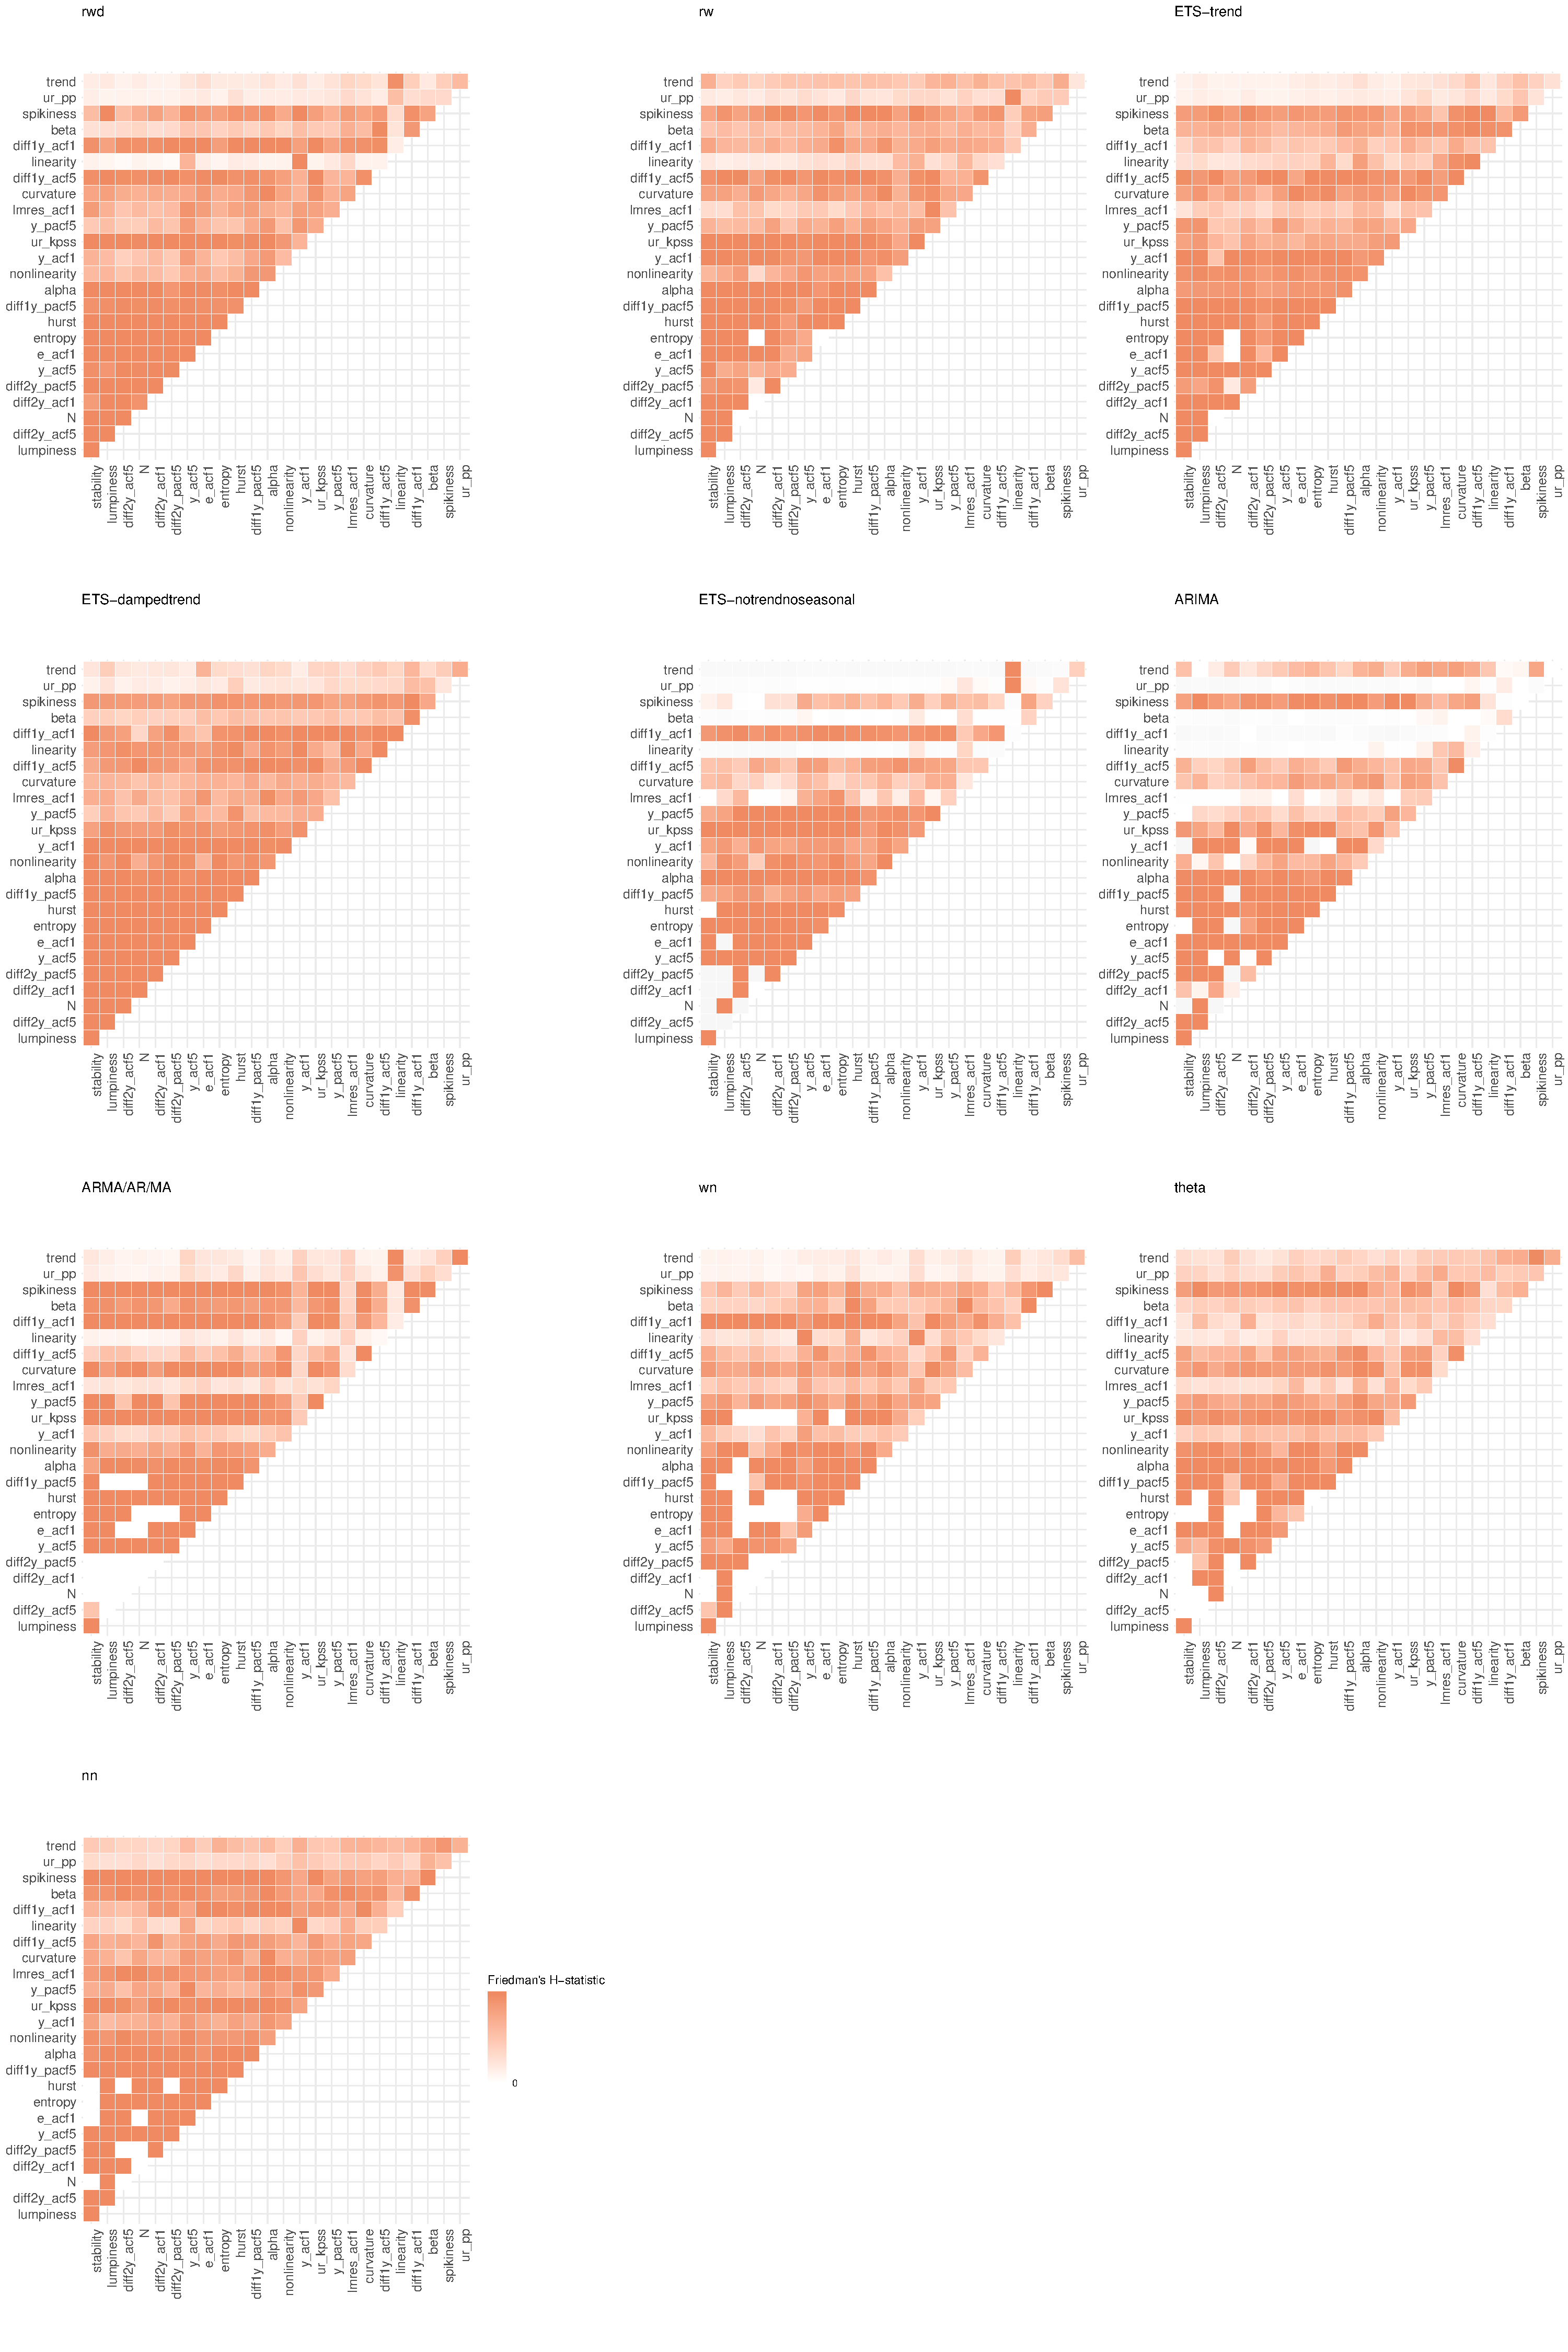
\includegraphics{figures/friedmany-1.pdf}
\caption{\label{fig:friedmany}The inteaction strength (Friedman's H-Statistic) for each feature with any other feature for yearly forest. The Hurst exponent within ETS\_DT has the highest interaction effect.}
\end{figure}

\begin{figure}
\centering
\includegraphics{figures/friedmanq-1.pdf}
\caption{\label{fig:friedmanq}The inteaction strength (Friedman's H-Statistic) for each feature with any other feature for quarterly forest. Top 5 interacting features are highlighted in purple. Stength of seasonality shows an extremely low interactivity within SARIMA, ETS\_DT and ETS\_DTS.}
\end{figure}

\begin{figure}
\centering
\includegraphics{figures/friedmanm-1.pdf}
\caption{\label{fig:friedmanm}The inteaction strength (Friedman's H-Statistic) for each feature with any other feature for quarterly forest. Top 5 interacting features are highlighted in purple. Curvature shows highest level of interactivity within ETS\_DTS}
\end{figure}

\begin{figure}[h]

{\centering \includegraphics{figures/friedmanw-1} 

}

\caption{The inteaction strength (Friedman's H-Statistic) for each feature with any other feature for weekly forest. Overall, the interaction effects between the features are very weak.}\label{fig:friedmanw}
\end{figure}

\begin{figure}[h]

{\centering \includegraphics{figures/friedmand-1} 

}

\caption{The inteaction strength (Friedman's H-Statistic) for each feature with any other feature for daily forest. Strength of trend shows highest level of interactivity within white noise class.}\label{fig:friedmand}
\end{figure}

\begin{figure}[h]

{\centering \includegraphics{figures/friedmanh-1} 

}

\caption{The inteaction strength (Friedman's H-Statistic) for each feature with any other feature for hourly forest. Linearity shows high level of interactivity within random walk with drift.}\label{fig:friedmanh}
\end{figure}

\clearpage

\printbibliography[title=References]

\end{document}
